\qrchapter{https://forgottenpillar.com/rsc/en-fp-chapter15}{Dr. Kellogg and the Trinity doctrine}


\qrchapter{https://forgottenpillar.com/rsc/en-fp-chapter15}{د. كيلوغ وعقيدة الثالوث}


The key problem with the Kellogg controversy was the sentiments over the \emcap{personality of God}, which were departing from the foundation of our faith, that God established at the beginning of our work. We have been told that \egwinline{Many things of like character will in the future arise}[Ms137-1903.10; 1903][https://egwwritings.org/read?panels=p9939.17]. In the book, the Living Temple, we see the sentiments regarding the \emcap{personality of God} and where His presence is, which were stepping off of the \emcap{Fundamental Principles}. This step was never supposed to be made! But we raise the question, where was this step heading? We will see the evidence that this step was heading toward the Trinity doctrine. Sister White prophesied that Kellogg’s step would lead toward the Omega heresy. Can we see the connection between Kellogg’s controversy and the Trinity doctrine?


كانت المشكلة الرئيسية في صراع كيلوغ هي الآراء حول \emcap{شخصانية الله}، والتي كانت تبتعد عن أساس إيماننا، الذي أسسه الله في بداية عملنا. لقد أُخبرنا أن \egwinline{العديد من الأمور المشابهة ستظهر في المستقبل}[Ms137-1903.10; 1903][https://egwwritings.org/read?panels=p9939.17]. في كتاب ذا ليفينغ تمبل، نرى الآراء المتعلقة بـ \emcap{شخصانية الله} وأين يوجد حضوره، والتي كانت خطوة بعيدًا عن \emcap{المبادئ الجوهرية}. هذه الخطوة لم يكن من المفترض أبدًا أن تُتخذ! لكننا نطرح السؤال، إلى أين كانت تتجه هذه الخطوة؟ سنرى الأدلة على أن هذه الخطوة كانت تتجه نحو عقيدة الثالوث. تنبأت الأخت وايت بأن خطوة كيلوغ ستؤدي إلى هرطقة أوميغا. هل يمكننا رؤية الصلة بين صراع كيلوغ وعقيدة الثالوث؟


In the following section, we want to present you with the connection between Kellogg’s controversy and the doctrine of Trinity. It is important to emphasize that the Living Temple does not contain this doctrine as it is believed today. The main problem with Kellogg’s teaching was the \textit{stepping off} of the \emcap{Fundamental Principles}, which were the foundation of our faith. The information we will present to you reveals that Dr. Kellogg justified his actions in stepping off of the foundation through his belief in the doctrine of Trinity. This is not difficult to see when we recognize that the \emcap{Fundamental Principles} were a non-Trinitarian. Our main focus should not be in recognizing the Trinity doctrine in Kellogg's arguments, but rather in understanding the differences between Kellogg’s teachings and the teachings of the \emcap{Fundamental Principles} regarding \egwinline{the personality of God and where His presence is}[SpTB02 51.3; 1903][https://egwwritings.org/read?panels=p417.262]. In other words, what were the steps Kellogg made in stepping off of the foundation of our faith? This approach is advocated by the Spirit of Prophecy and it will help us to avoid speculations regarding Kellogg’s motives—it will help us to focus upon the truth. Ellen White tells us that there are many good things written in the Living Temple, but they are mingled with specious, deceptive theories regarding the \emcap{personality of God} and \emcap{of Christ}.


في القسم التالي، نريد أن نقدم لكم الصلة بين صراع كيلوغ وعقيدة الثالوث. من المهم التأكيد على أن كتاب ذا ليفينغ تمبل لا يحتوي على هذه العقيدة كما يُعتقد اليوم. المشكلة الرئيسية في تعاليم كيلوغ كانت \textit{الابتعاد} عن \emcap{المبادئ الجوهرية}، التي كانت أساس إيماننا. المعلومات التي سنقدمها لكم تكشف أن د. كيلوغ برر أفعاله في الابتعاد عن الأساس من خلال إيمانه بعقيدة الثالوث. هذا ليس من الصعب رؤيته عندما ندرك أن \emcap{المبادئ الجوهرية} كانت غير ثالوثية. يجب ألا يكون تركيزنا الرئيسي في التعرف على عقيدة الثالوث في حجج كيلوغ، بل في فهم الاختلافات بين تعاليم كيلوغ وتعاليم \emcap{المبادئ الجوهرية} فيما يتعلق بـ \egwinline{شخصانية الله وأين يوجد حضوره}[SpTB02 51.3; 1903][https://egwwritings.org/read?panels=p417.262]. بعبارة أخرى، ما هي الخطوات التي اتخذها كيلوغ في الابتعاد عن أساس إيماننا؟ هذا النهج تدعمه روح النبوة وسيساعدنا على تجنب التكهنات بشأن دوافع كيلوغ - سيساعدنا على التركيز على الحقيقة. تخبرنا إلين وايت أن هناك العديد من الأشياء الجيدة المكتوبة في ذا ليفينغ تمبل، لكنها ممزوجة بنظريات خادعة ومضللة فيما يتعلق بـ \emcap{شخصانية الله} و \emcap{المسيح}.


\begin{figure}[hp]
    \centering
    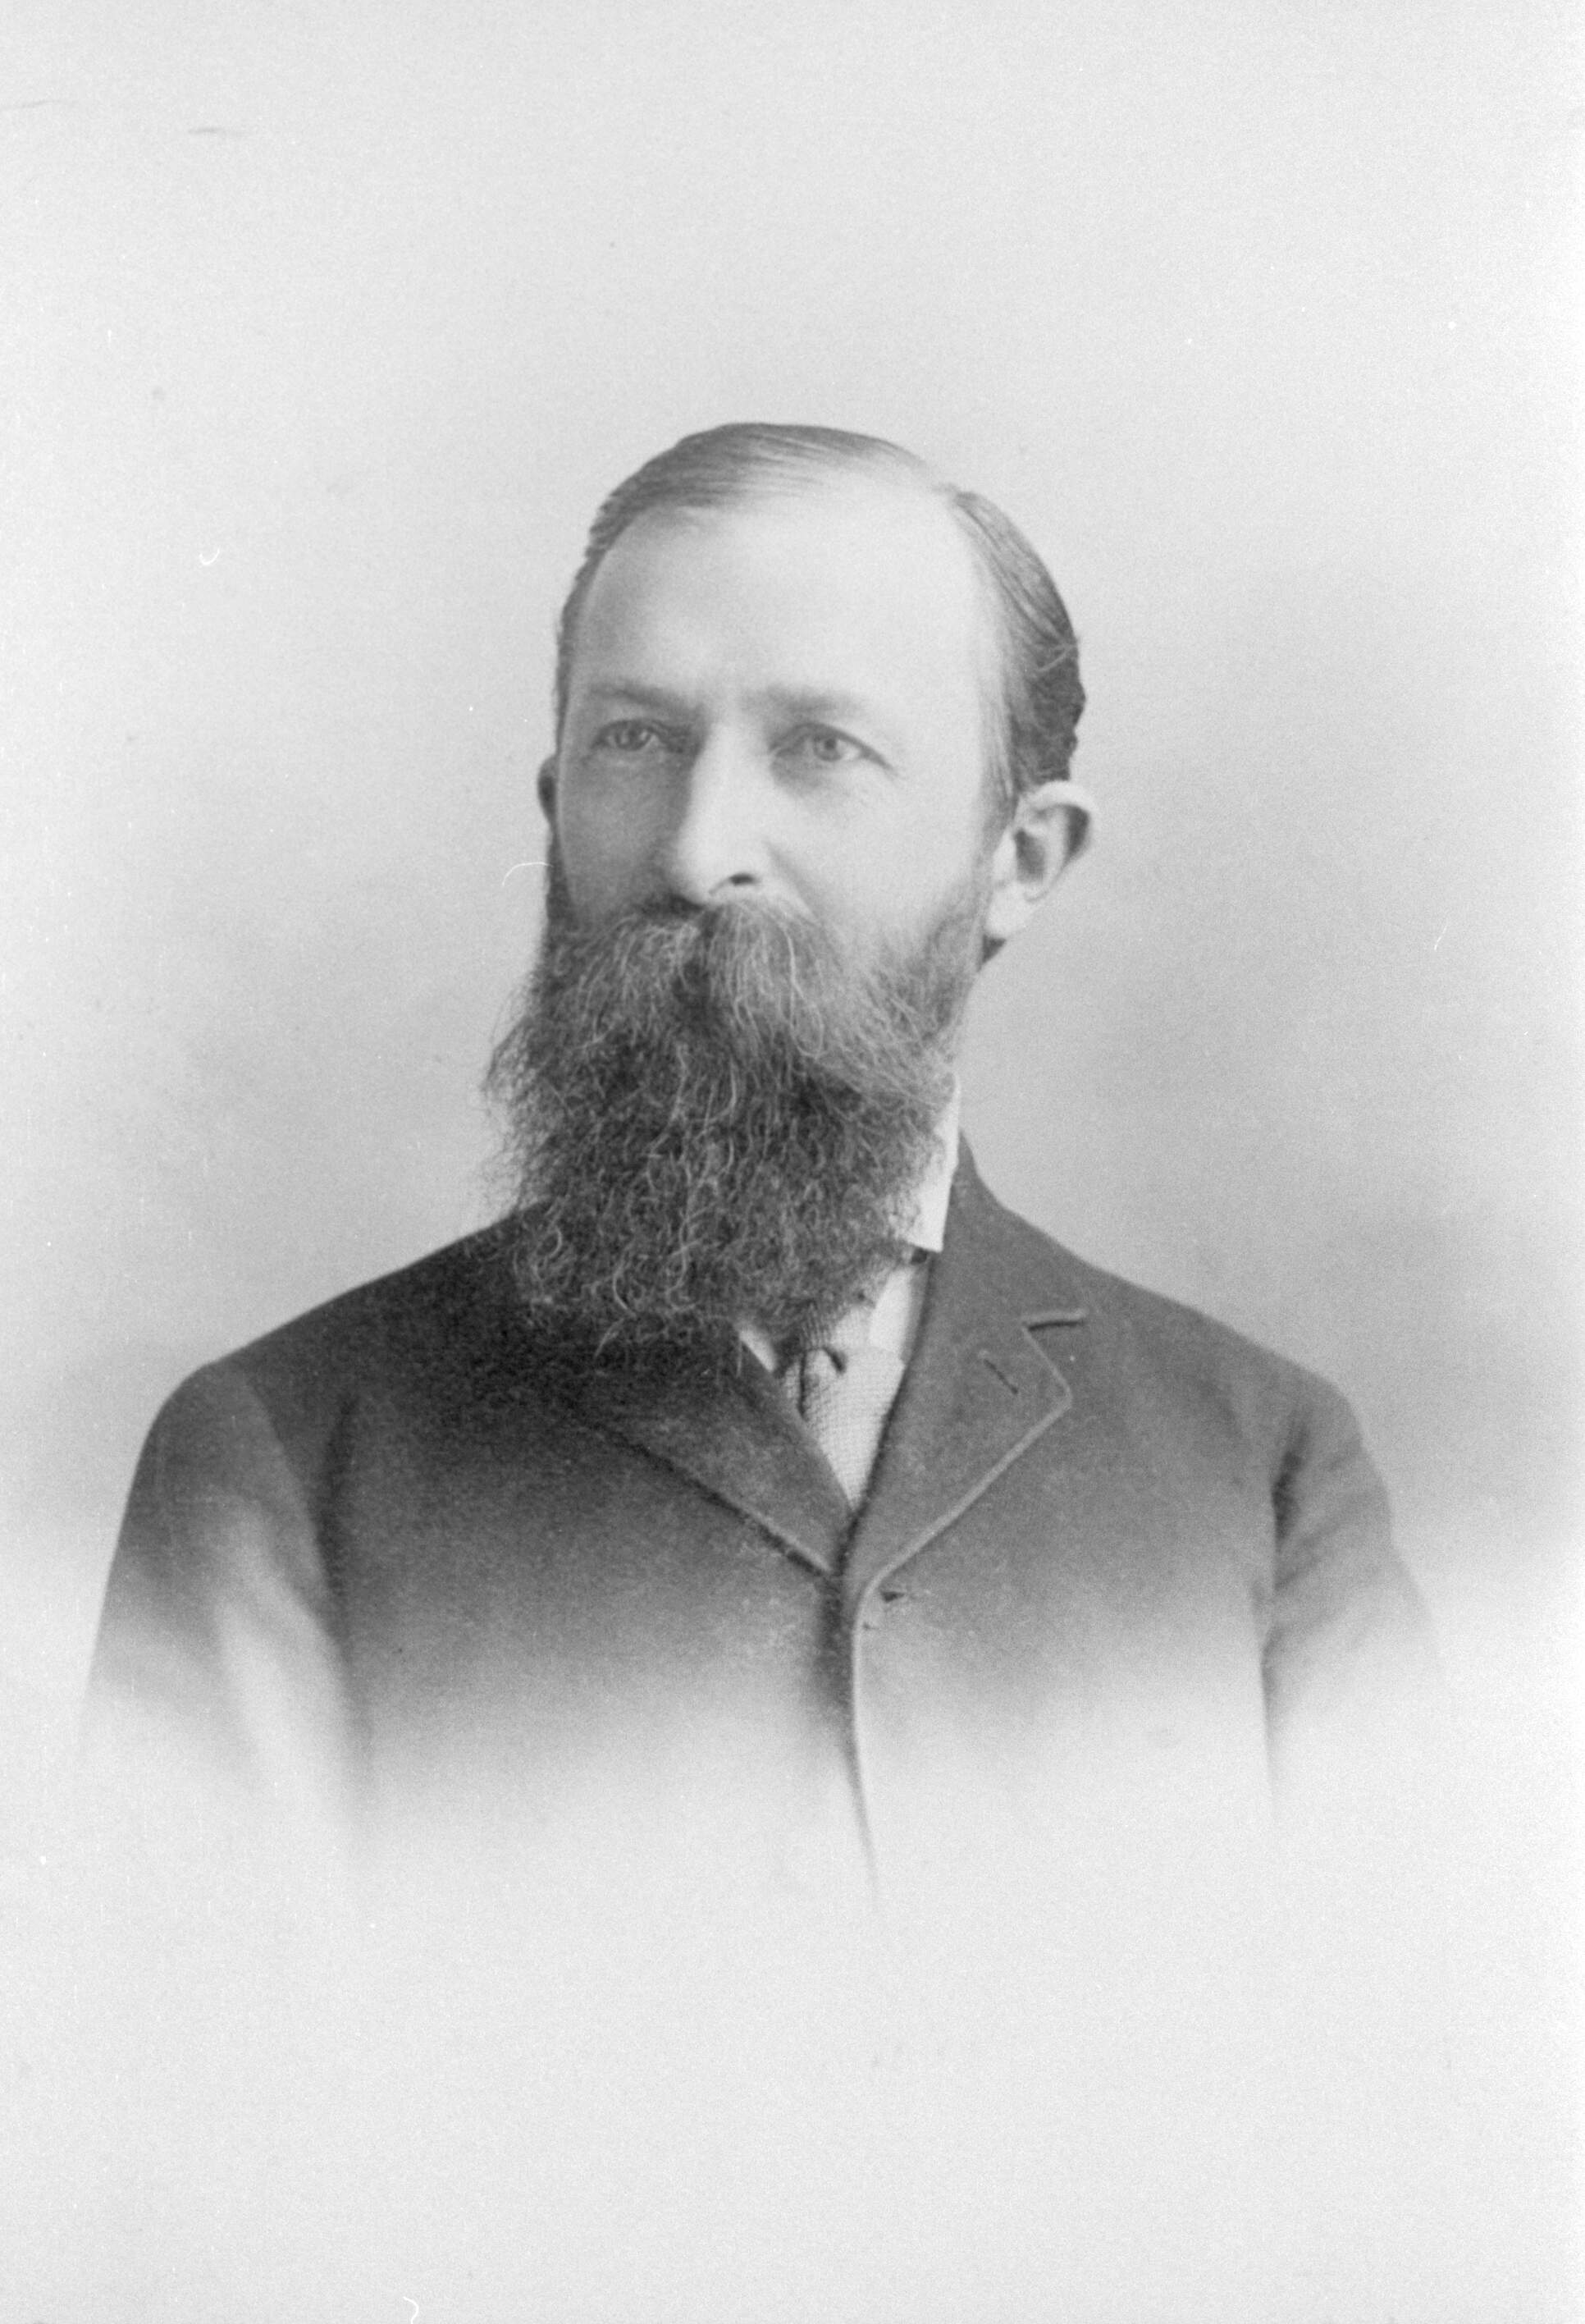
\includegraphics[width=1\linewidth]{images/john-h-kellogg.jpg}
    \caption*{John Harvey Kellogg (1852-1943)}
    \label{fig:john-h-kellogg}
\end{figure}


\begin{figure}[hp]
    \centering
    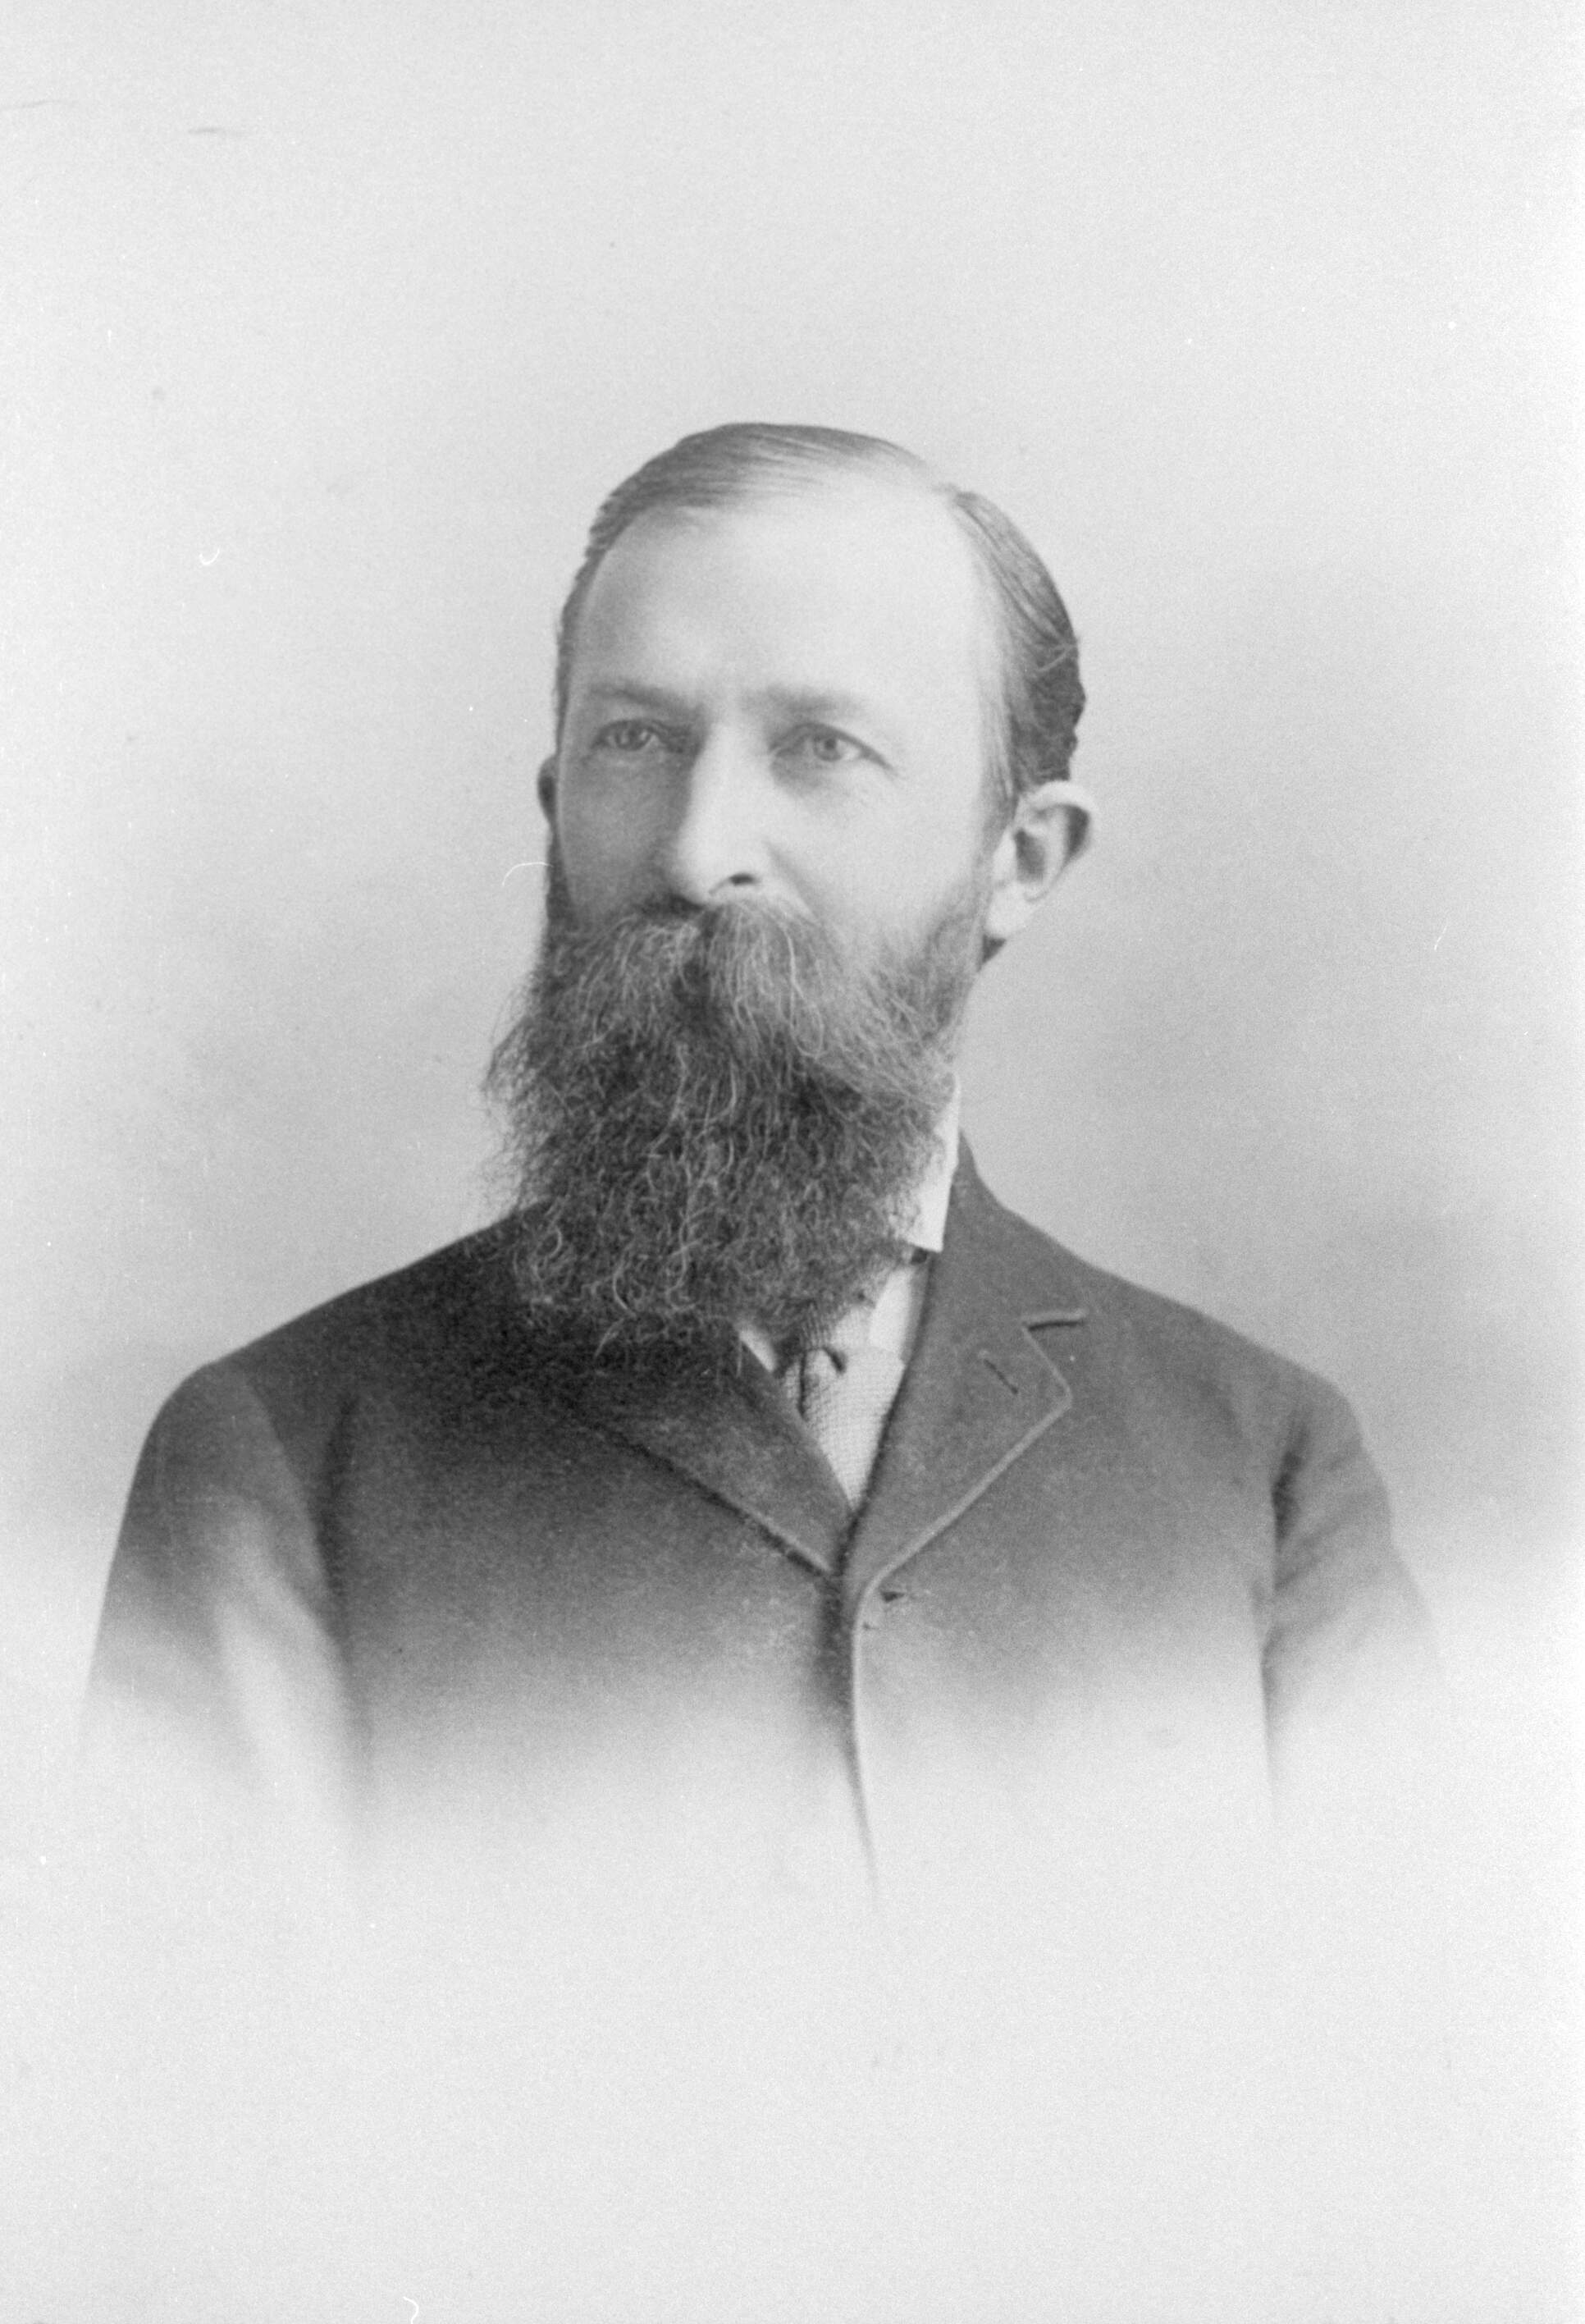
\includegraphics[width=1\linewidth]{images/john-h-kellogg.jpg}
    \caption*{جون هارفي كيلوغ (1852-1943)}
    \label{fig:john-h-kellogg}
\end{figure}


\egw{\textbf{The book Living Temple contains specious, \underline{deceptive sentiments regarding the personality of God and of Christ}}. The Lord opened before me the true meaning of these sentiments, showing me that unless they were steadfastly repudiated, they would deceive the very elect. \textbf{Precious truth and beautiful sentiments were woven in with false, misleading theories. Thus truth was used to substantiate the \underline{most dangerous errors}. The precious representations of God are so misconstrued as to appear to uphold falsehoods \underline{originated by the great apostate}. Sentiments that belong to the revealings of God are mingled with specious, deceptive theories of satanic agencies}.}[Lt146-1905.2; 1905][https://egwwritings.org/read?panels=p9430.8]


\egw{\textbf{كتاب ذا ليفينغ تمبل يحتوي على آراء خادعة \underline{ومضللة بخصوص شخصانية الله والمسيح}}. لقد كشف الرب أمامي المعنى الحقيقي لهذه الآراء، وأظهر لي أنه ما لم يتم رفضها بثبات، فإنها ستخدع المختارين أنفسهم. \textbf{لقد تم نسج حقائق ثمينة وآراء جميلة مع نظريات كاذبة ومضللة. وهكذا استُخدمت الحقيقة لدعم \underline{أخطر الأخطاء}. تم تفسير التمثيلات الثمينة لله بشكل خاطئ لتبدو وكأنها تدعم الأكاذيب \underline{التي نشأت من المرتد العظيم}. الآراء التي تنتمي إلى إعلانات الله ممزوجة بنظريات خادعة ومضللة من وكالات شيطانية}.}[Lt146-1905.2; 1905][https://egwwritings.org/read?panels=p9430.8]


\egwnogap{In the controversy over these theories \textbf{it has been asserted that I believed and taught the same things} that I have been instructed to condemn in the book Living Temple. \textbf{This I deny}. In the name of Jesus Christ of Nazareth, \textbf{I say that this is not so}.}[Lt146-1905.3; 1905][https://egwwritings.org/read?panels=p9430.9]


\egwnogap{في الجدل حول هذه النظريات \textbf{تم الادعاء بأنني آمنت وعلّمت نفس الأشياء} التي تلقيت تعليمات بإدانتها في كتاب ذا ليفينغ تمبل. \textbf{أنا أنكر ذلك}. باسم يسوع المسيح الناصري، \textbf{أقول إن هذا غير صحيح}.}[Lt146-1905.3; 1905][https://egwwritings.org/read?panels=p9430.9]


This mixture of truth and error makes the matter difficult. In the eyes of pro-trinitarian scholars, the problem is solely attributed to pantheism, and the evidence of Kellogg's belief in the Trinity doctrine is interpreted as belief in a false Trinity\footnote{Whidden, Woodrow W, et al. \textit{The Trinity : Understanding God's Love, His Plan of Salvation, and Christian Relationships}. Hagerstown, Md, Review And Herald Pub. Association, 2002., p. 217}. Sister White's rebuke is attributed to the defense of the “correct” Trinity, which she supposedly believed. Unfortunately, such interpretation does not acknowledge Sister White's defense of the \emcap{Fundamental Principles} regarding the \emcap{personality of God} and of Christ, thus it is a misinterpretation of her work. In the following sections, we will examine historical data on Dr. Kellogg's connection with the doctrine of Trinity from the perspective of the Adventist truth on the \emcap{personality of God}, which constituted the foundation of our faith. With this perspective, we believe that the historical data will shine in a new light and spark honest and constructive dialogue in our church.


هذا المزيج من الحق والخطأ يجعل الأمر صعبًا. في نظر العلماء المؤيدين للثالوث، تُعزى المشكلة فقط إلى وحدة الوجود، ويُفسر دليل إيمان كيلوغ بعقيدة الثالوث على أنه إيمان بثالوث زائف\footnote{Whidden, Woodrow W, et al. \textit{The Trinity : Understanding God's Love, His Plan of Salvation, and Christian Relationships}. Hagerstown, Md, Review And Herald Pub. Association, 2002., p. 217}. يُنسب توبيخ الأخت وايت إلى الدفاع عن الثالوث “الصحيح”، الذي يُفترض أنها آمنت به. للأسف، مثل هذا التفسير لا يعترف بدفاع الأخت وايت عن \emcap{المبادئ الجوهرية} فيما يتعلق بـ \emcap{شخصانية الله} والمسيح، وبالتالي فهو تفسير خاطئ لعملها. في الأقسام التالية، سندرس البيانات التاريخية حول علاقة د. كيلوغ بعقيدة الثالوث من منظور الحقيقة الأدفنتستية حول \emcap{شخصانية الله}، التي شكلت أساس إيماننا. بهذا المنظور، نعتقد أن البيانات التاريخية ستتألق بنور جديد وتثير حوارًا صادقًا وبناءً في كنيستنا.


\section*{Correspondence of Dr. Kellogg and Brother Butler}


\section*{مراسلات د. كيلوغ والأخ بتلر}


In the following section we briefly present you with the well-known correspondence between Dr. Kellogg and G. I. Butler over the book, the Living Temple. Here, we see Dr. Kellogg’s objections regarding the controversy. He wrote to Brother Butler:


في القسم التالي نقدم لكم بإيجاز المراسلات المعروفة بين د. كيلوغ وج. آي. بتلر حول كتاب ذا ليفينغ تمبل. هنا، نرى اعتراضات د. كيلوغ بخصوص الصراع. كتب إلى الأخ بتلر:


\others{As far as I can fathom, the \textbf{difficulty }which is found \textbf{in ‘The Living Temple’,} \textbf{the whole thing may be simmered down to the question}: \textbf{\underline{Is the Holy Ghost a person}?} You say no. I had supposed the Bible said this for the reason that the personal pronoun ‘he’ is used in speaking of the Holy Ghost. \textbf{Sister White uses the pronoun ‘he’ and has said in so many words that the Holy Ghost is \underline{the third person of the Godhead}}. \textbf{How the Holy Ghost can be the third person and not be a person at all is difficult for me to see}.}[Letter: J. H. Kellogg to G. I. Butler. Oct 28. 1903][https://static1.squarespace.com/static/554c4998e4b04e89ea0c4073/t/5db9fbc96defed1e45b497a4/1572469707862/1903-10-28-Kellog-to-Butler.pdf]


\others{بقدر ما أستطيع أن أفهم، \textbf{الصعوبة} التي توجد \textbf{في ‘ذا ليفينغ تمبل’،} \textbf{يمكن تلخيص الأمر كله في السؤال}: \textbf{\underline{هل الروح القدس شخص}؟} أنت تقول لا. كنت أفترض أن الكتاب المقدس قال هذا لسبب أن الضمير الشخصي ‘هو’ يُستخدم عند الحديث عن الروح القدس. \textbf{الأخت وايت تستخدم الضمير ‘هو’ وقالت بكلمات واضحة أن الروح القدس هو \underline{الشخص الثالث في اللاهوت}}. \textbf{كيف يمكن للروح القدس أن يكون الشخص الثالث وليس شخصًا على الإطلاق، هذا أمر يصعب علي فهمه}.}[Letter: J. H. Kellogg to G. I. Butler. Oct 28. 1903][https://static1.squarespace.com/static/554c4998e4b04e89ea0c4073/t/5db9fbc96defed1e45b497a4/1572469707862/1903-10-28-Kellog-to-Butler.pdf]


\begin{figure}[hp]
    \centering
    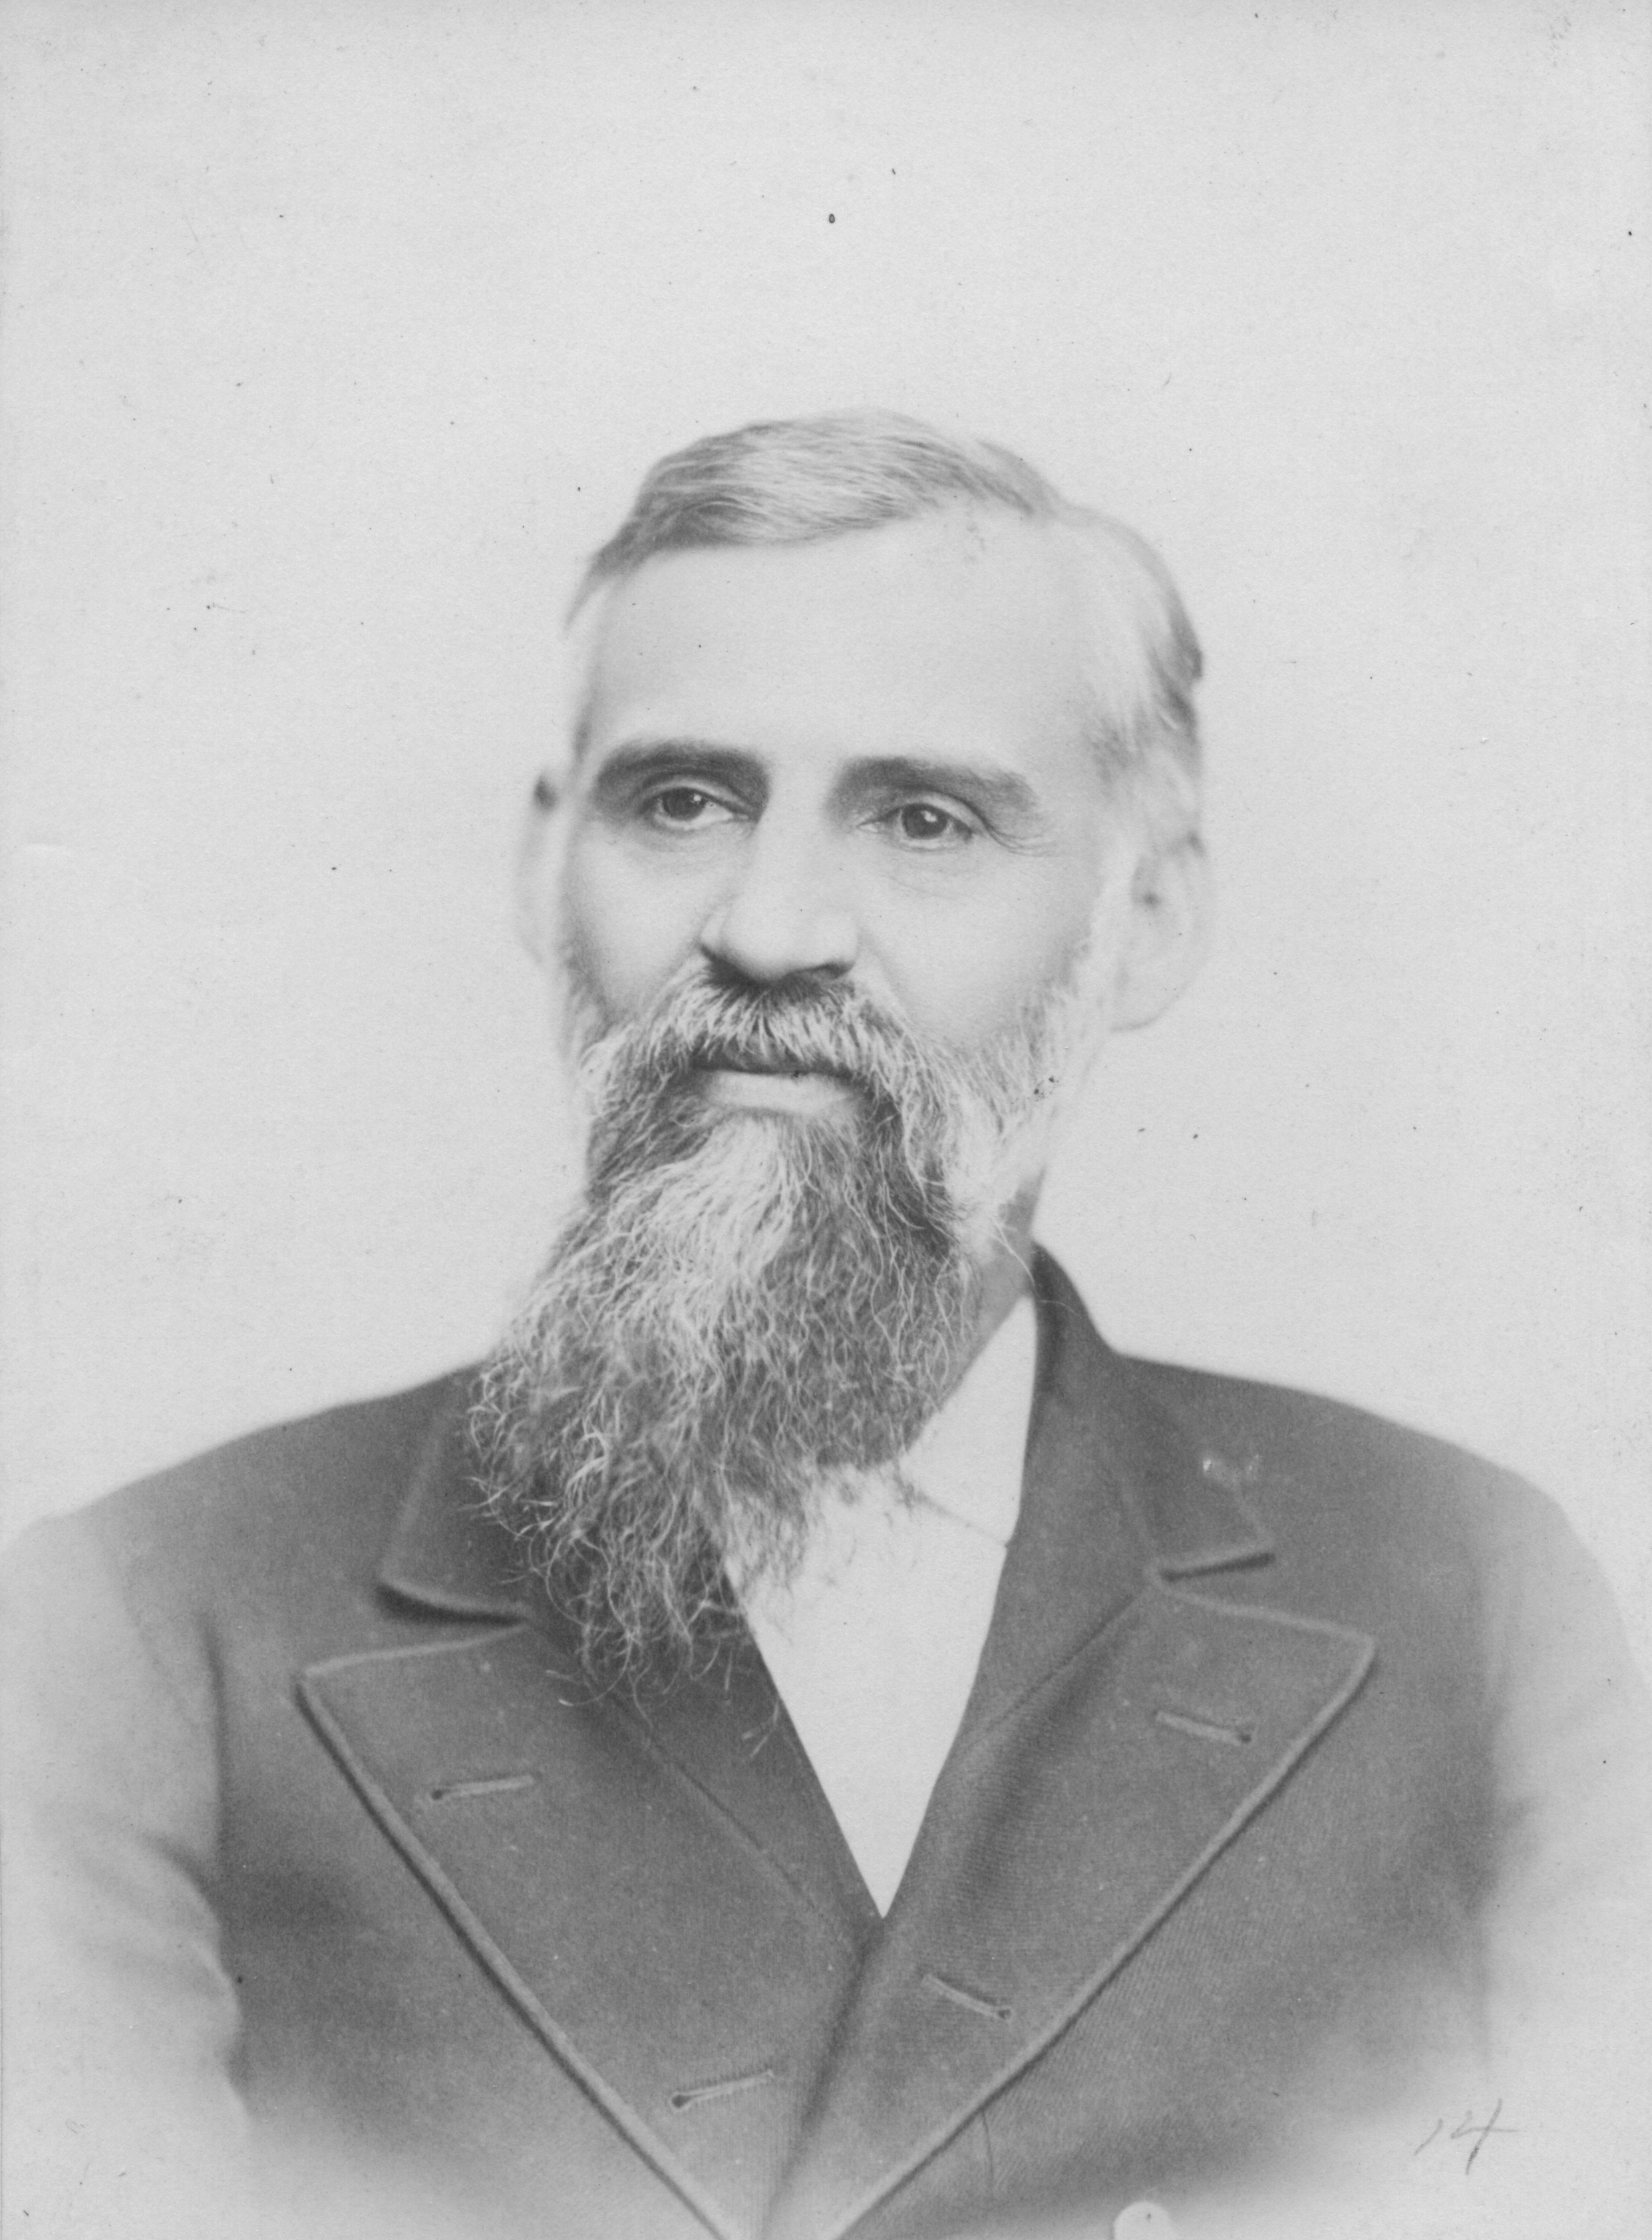
\includegraphics[width=1\linewidth]{images/george-ide-butler.jpg}
    \caption*{George Ide Butler (1834-1918)}
    \label{fig:g-i-butler}
\end{figure}


\begin{figure}[hp]
    \centering
    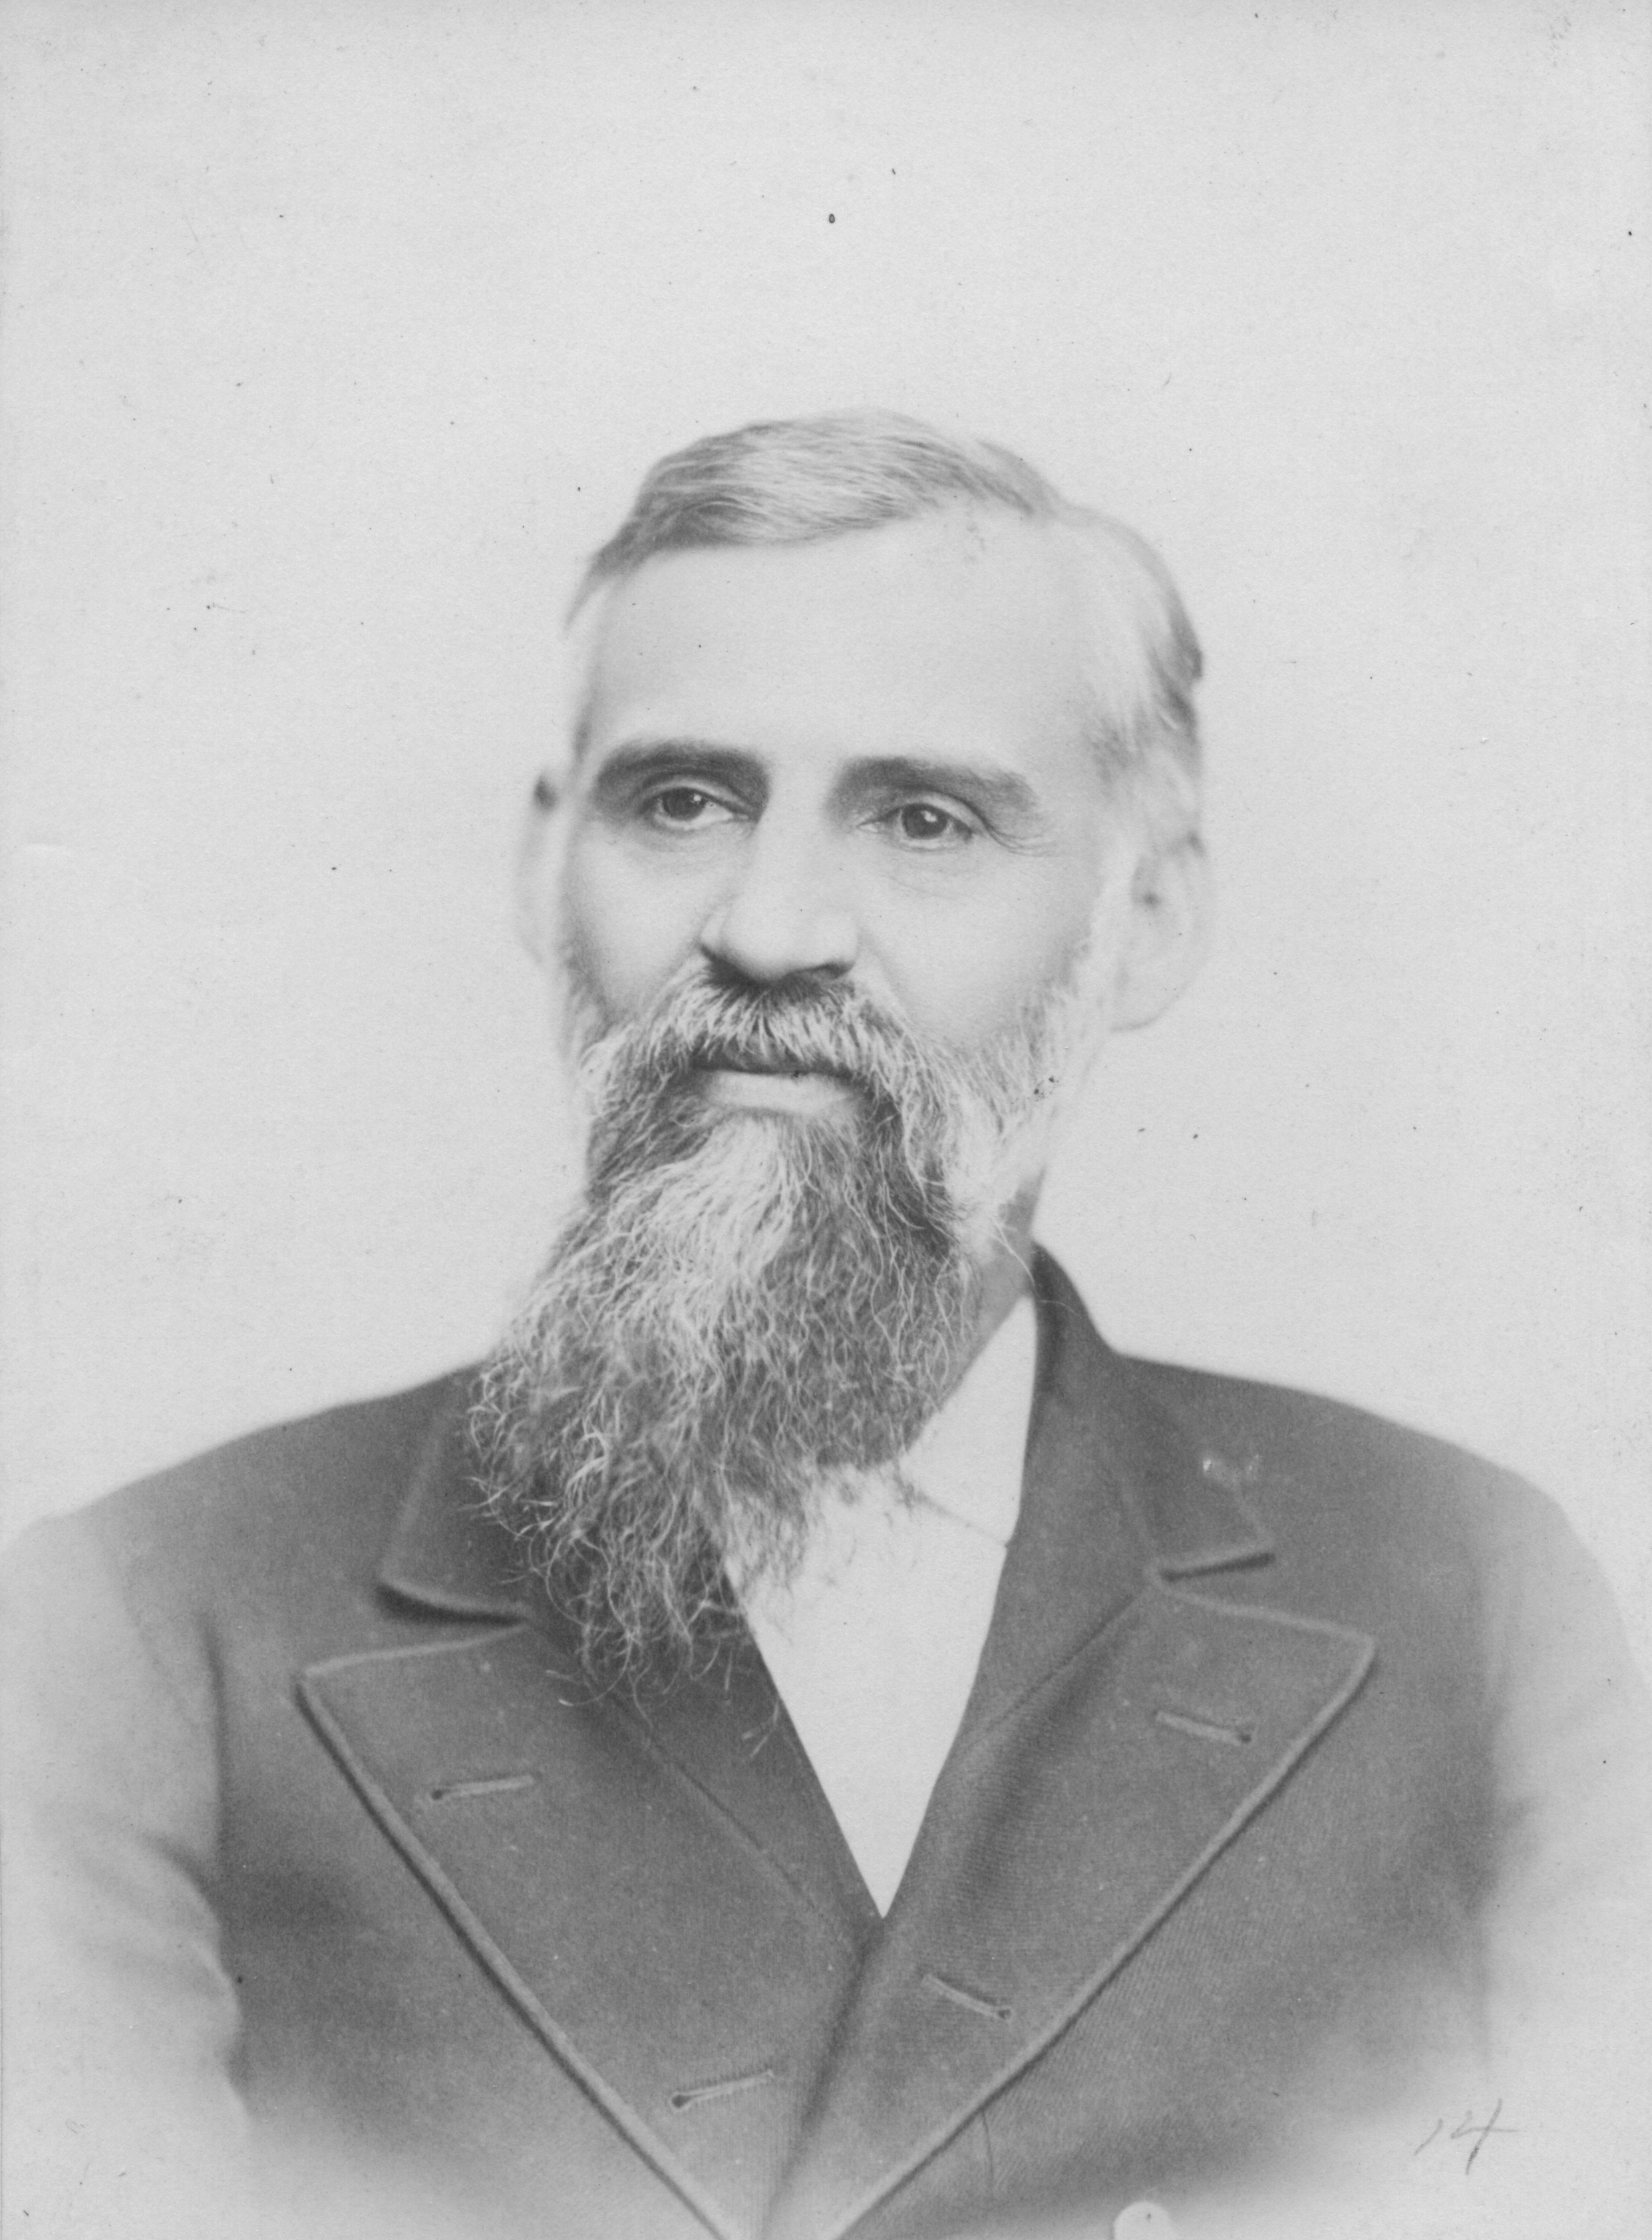
\includegraphics[width=1\linewidth]{images/george-ide-butler.jpg}
    \caption*{جورج آيد بتلر (1834-1918)}
    \label{fig:g-i-butler}
\end{figure}


According to Dr. Kellogg’s perspective, the whole problem with the book ‘The Living Temple’ comes down to the question “\textit{Is the Holy Ghost a person?}”. Obviously, he does not advocate an impersonal God, as he is often accused of\footnote{Whidden, Woodrow W, et al. \textit{The Trinity : Understanding God's Love, His Plan of Salvation, and Christian Relationships}. Hagerstown, Md, Review And Herald Pub. Association, 2002., p. 217}. Moreover, he even believes that the Holy Ghost is a \textit{third person of the Godhead}. Also, he claims that Brother Butler does not believe that the Holy Ghost is a person. The problem obviously lies in the definition of the word \textit{‘person’}. On this point, Kellogg continues:


وفقًا لوجهة نظر الدكتور كيلوغ، فإن المشكلة الكاملة مع كتاب “ذا ليفينغ تمبل” تتلخص في سؤال “\textit{هل الروح القدس شخص؟}”. من الواضح أنه لا يدعو إلى إله غير شخصي، كما يُتهم غالبًا\footnote{Whidden, Woodrow W, et al. \textit{The Trinity : Understanding God's Love, His Plan of Salvation, and Christian Relationships}. Hagerstown, Md, Review And Herald Pub. Association, 2002., p. 217}. علاوة على ذلك، فهو يعتقد أن الروح القدس هو \textit{الشخص الثالث في اللاهوت}. كما يدعي أن الأخ بتلر لا يؤمن بأن الروح القدس هو شخص. المشكلة تكمن بوضوح في تعريف كلمة \textit{‘شخص’}. وفي هذه النقطة، يواصل كيلوغ:


\others{I believe this Spirit of God to be a personality you don’t. But this is purely a question of definition. \textbf{I believe the Spirit of God is a personality}; you say, No, it is not a personality. Now the only reason why we differ is because we \textbf{differ in our ideas as to \underline{what a personality is}}. \textbf{Your idea of personality is perhaps that of \underline{semblance to a person} or a human being}.}[Letter: J. H. Kellogg to G. I. Butler. Oct 28. 1903][https://static1.squarespace.com/static/554c4998e4b04e89ea0c4073/t/5db9fbc96defed1e45b497a4/1572469707862/1903-10-28-Kellog-to-Butler.pdf]


\others{أنا أؤمن بأن روح الله هذا هو شخصية وأنت لا تؤمن بذلك. لكن هذه مسألة تعريف بحتة. \textbf{أنا أؤمن أن روح الله هو شخصية}؛ أنت تقول، لا، إنه ليس شخصية. الآن السبب الوحيد لاختلافنا هو أننا \textbf{نختلف في أفكارنا حول \underline{ماهية الشخصية}}. \textbf{فكرتك عن الشخصية ربما تكون \underline{المشابهة لشخص} أو كائن بشري}.}[Letter: J. H. Kellogg to G. I. Butler. Oct 28. 1903][https://static1.squarespace.com/static/554c4998e4b04e89ea0c4073/t/5db9fbc96defed1e45b497a4/1572469707862/1903-10-28-Kellog-to-Butler.pdf]


Brother Butler replied:


رد الأخ بتلر:


\others{\textbf{So far as Sister White and you being in perfect agreement, I shall have to leave that entirely between you and Sister White. \underline{Sister White says there is not perfect agreement; you claim there is}. \underline{I know some of her remarks seem to give you strong ground for claiming that she does}. I am candid enough to say that, but I must give her the credit until she disowns it of saying there is a difference too, and I do not believe you can fully tell just what she means. \underline{God dwells in us by His Holy Spirit}, as a Comforter, as a Reprover, especially the former. When we come to Him we partake of Him in that sense, because the Spirit comes forth from Him; \underline{it comes forth from the Father and the Son}. It is not a person walking around on foot, or flying \underline{as a literal being}, \underline{in any such sense as Christ and the Father are} – at least, if it is, it is utterly beyond my comprehension of the meaning of language or words}.}[Letter: G. I. Butler to J. H. Kellogg. April 5. 1904]


\others{\textbf{بقدر ما يتعلق الأمر بالأخت وايت وأنت في اتفاق تام، سأضطر إلى ترك ذلك بالكامل بينك وبين الأخت وايت. \underline{الأخت وايت تقول إنه لا يوجد اتفاق تام؛ أنت تدعي أنه يوجد}. \underline{أعلم أن بعض ملاحظاتها تبدو أنها تمنحك أرضية قوية للادعاء بأنها كذلك}. أنا صريح بما يكفي لأقول ذلك، لكن يجب أن أمنحها الفضل حتى تتنصل من قولها إن هناك اختلافًا أيضًا، ولا أعتقد أنك تستطيع أن تخبر بالضبط ما تعنيه. \underline{الله يسكن فينا بروحه القدس}، كمعزٍ، وكموبخ، وخاصة الأول. عندما نأتي إليه نشترك فيه بهذا المعنى، لأن الروح يخرج منه؛ \underline{إنه يخرج من الآب والابن}. إنه ليس شخصًا يمشي على قدميه، أو يطير \underline{ككائن حرفي}، \underline{بأي معنى كما هو المسيح والآب} - على الأقل، إذا كان كذلك، فهو خارج نطاق فهمي تمامًا لمعنى اللغة أو الكلمات}.}[Letter: G. I. Butler to J. H. Kellogg. April 5. 1904]


The given correspondence is crucial for understanding the Kellogg controversy. Kellogg himself stated, \others{the whole thing may be simmered down to the question: \textbf{Is the Holy Ghost a person?}} Similarly Dr. Kellogg wrote to William White: \others{I have been studying very carefully to see what is \textbf{the real root of the difficulty with the Living Temple}, and as far as I can see \textbf{\underline{the whole question} resolves itself into this: \underline{Is the Holy Ghost, a person}?}}[Letter J. H. Kellogg to William White, October 28, 1903][https://drive.google.com/file/d/1\_S4S-Hc0K7Ka8gda9oRhPuAb9XzBTwmb/view] How does Kellogg's conclusion compare to the review and instruction of heavenly origin, which clearly told us that the reasoning in the Living Temple is \egwinline{naught but speculation in regard to \textbf{the personality of God and where His presence is}}[SpTB02 51.3; 1904][https://egwwritings.org/read?panels=p417.262]? In the writings of Ellen White and the pioneers, the term ‘\textit{personality of God}’ refers specifically to the personality of the Father. So, why does Kellogg claim that the real issue is the personality of the Holy Spirit, when God indicated that the issue concerns the personality of the Father?


المراسلات المذكورة حاسمة لفهم صراع كيلوغ. صرح كيلوغ نفسه، \others{يمكن تلخيص الأمر كله في السؤال: \textbf{هل الروح القدس شخص؟}} وبالمثل كتب الدكتور كيلوغ إلى ويليام وايت: \others{لقد كنت أدرس بعناية شديدة لمعرفة ما هو \textbf{الجذر الحقيقي للصعوبة مع كتاب ذا ليفينغ تمبل}، وبقدر ما أستطيع أن أرى \textbf{\underline{المسألة بأكملها} تتلخص في هذا: \underline{هل الروح القدس شخص}؟}}[Letter J. H. Kellogg to William White, October 28, 1903][https://drive.google.com/file/d/1\_S4S-Hc0K7Ka8gda9oRhPuAb9XzBTwmb/view] كيف يقارن استنتاج كيلوغ بالمراجعة والتعليمات ذات الأصل السماوي، التي أخبرتنا بوضوح أن المنطق في كتاب ذا ليفينغ تمبل هو \egwinline{ليس سوى تكهنات فيما يتعلق \textbf{بشخصانية الله وأين يوجد حضوره}}[SpTB02 51.3; 1904][https://egwwritings.org/read?panels=p417.262]؟ في كتابات إلين وايت والرواد، يشير مصطلح ‘\textit{شخصانية الله}’ تحديدًا إلى شخصانية الآب. إذن، لماذا يدعي كيلوغ أن القضية الحقيقية هي شخصانية الروح القدس، بينما أشار الله إلى أن القضية تتعلق بشخصانية الآب؟


Many assume that Dr. Kellogg is being manipulative, evading the core issue. However, under a particular premise, his arguments concerning the personality of the Holy Spirit logically support his controversial views on the \emcap{personality of God}. This premise becomes evident within the data itself when we closely follow his reasoning.


يفترض الكثيرون أن الدكتور كيلوغ يتلاعب، متجنبًا القضية الأساسية. ومع ذلك، في ظل فرضية معينة، فإن حججه المتعلقة بشخصانية الروح القدس تدعم منطقيًا آراءه المثيرة للجدل حول \emcap{شخصانية الله}. تصبح هذه الفرضية واضحة ضمن البيانات نفسها عندما نتتبع منطقه عن كثب.


As we have seen earlier, the doctrine on the \emcap{personality of God} teaches that God, the Father, possesses a form—a tangible, material body. Dr. Kellogg concurred that this assertion holds true within the bounds of our finite conception of God\footnote{\href{https://archive.org/details/J.H.Kellogg.TheLivingTemple1903/page/n33/}{Dr. John H. Kellogg, The Living Temple, p.31.}}. However, he argued that, in reality, God transcends our conceptions regarding His form, as He is beyond the constraints of space\footnote{\href{https://archive.org/details/J.H.Kellogg.TheLivingTemple1903/page/n33/}{Dr. John H. Kellogg, The Living Temple, p.33.}}. In this sense, Kellogg effectively does away with the reality of God’s physical, material body. The premise that would validate Dr. Kellogg’s viewpoint is the \textit{exclusive equivalence} in understanding the \emcap{personality of God} and that of the Holy Spirit. Is the Holy Spirit constrained by space? No, He is not. Does the Holy Spirit have a physical body? No! According to Jesus, \bible{for a spirit hath not flesh and bones}[Luke 24:39]. Is the Holy Ghost a person? The answer hinges on our interpretation of what it means to be a person. What is that quality or state of the Holy Spirit being a person?\footnote{Direct application of the definition on the word ‘\textit{personality}’ from the \href{https://www.merriam-webster.com/dictionary/personality}{Merriam Webster Dictionary}} When comparing Dr. Kellogg's belief in the personality of the Holy Spirit with Brother Butler's views, it becomes evident that the quality of the Holy Spirit being a person does not align with \others{that of \textbf{semblance to a person} or a human being}. Butler explicitly stated his criteria for this determination\footnote{In his letter to Dr. Kellogg, Brother Butler further asserted that there is no distinction between the person and the bodily presence. See \href{https://c7da.us/egwdl/Butler\%20to\%20Kellogg\%20Aug121904.pdf}{Letter from Butler to Kellogg, August 12, 1904, p.6}}: \others{\textbf{It is not a person walking around on foot, or flying \underline{as a literal being}, \underline{in any such sense as Christ and the Father are} – at least, if it is, it is utterly beyond my comprehension of the meaning of language or words}}.


كما رأينا سابقًا، تعلم عقيدة \emcap{شخصانية الله} أن الله، الآب، يمتلك شكلاً - جسدًا ماديًا ملموسًا. وافق الدكتور كيلوغ على أن هذا التأكيد صحيح ضمن حدود تصورنا المحدود لله\footnote{\href{https://archive.org/details/J.H.Kellogg.TheLivingTemple1903/page/n33/}{Dr. John H. Kellogg, The Living Temple, p.31.}}. ومع ذلك، جادل بأن الله في الواقع يتجاوز تصوراتنا بشأن شكله، لأنه يتجاوز قيود المكان\footnote{\href{https://archive.org/details/J.H.Kellogg.TheLivingTemple1903/page/n33/}{Dr. John H. Kellogg, The Living Temple, p.33.}}. بهذا المعنى، يتخلص كيلوغ بشكل فعال من واقع جسد الله المادي الفيزيائي. الفرضية التي من شأنها أن تصادق على وجهة نظر الدكتور كيلوغ هي \textit{التكافؤ الحصري} في فهم \emcap{شخصانية الله} وشخصانية الروح القدس. هل الروح القدس مقيد بالمكان؟ لا، ليس كذلك. هل للروح القدس جسد مادي؟ لا! وفقًا ليسوع، \bible{فَإِنَّ الرُّوحَ لَيْسَ لَهُ لَحْمٌ وَعِظَامٌ}[لوقا 24:39]. هل الروح القدس شخص؟ الإجابة تعتمد على تفسيرنا لما يعنيه أن تكون شخصًا. ما هي الصفة أو الحالة التي يكون بها الروح القدس شخصًا؟\footnote{تطبيق مباشر للتعريف على كلمة ‘\textit{شخصانية}’ من \href{https://www.merriam-webster.com/dictionary/personality}{قاموس ميريام ويبستر}} عند مقارنة إيمان الدكتور كيلوغ بشخصانية الروح القدس مع آراء الأخ بتلر، يتضح أن صفة كون الروح القدس شخصًا لا تتوافق مع \others{صفة \textbf{المشابهة لشخص} أو كائن بشري}. صرح بتلر صراحة بمعاييره لهذا التحديد\footnote{في رسالته إلى الدكتور كيلوغ، أكد الأخ بتلر أيضًا أنه لا يوجد تمييز بين الشخص والحضور الجسدي. انظر \href{https://c7da.us/egwdl/Butler\%20to\%20Kellogg\%20Aug121904.pdf}{Letter from Butler to Kellogg, August 12, 1904, p.6}}: \others{\textbf{إنه ليس شخصًا يمشي على قدميه، أو يطير \underline{ككائن حرفي}، \underline{بأي معنى كما هو المسيح والآب} - على الأقل، إذا كان كذلك، فهو خارج نطاق فهمي تمامًا لمعنى اللغة أو الكلمات}}.


Have you noticed that Brother Butler addressed Kellogg’s unspoken premise? Butler drew a distinction between the Father and Christ, in relation to the Holy Spirit. Brother Butler is correct. There exists a contrast between the personality of the Holy Spirit and that of God and Christ. Christ and the Father possess a physical form of a person, whereas the Holy Spirit does not. To do away with the physical form of a person of the Father is to \textit{exclusively equate} the understanding of the personality of the Father with that of the Holy Spirit. Kellogg’s approach is compelling, because it was backed by valid arguments regarding the personality of the Holy Spirit.


هل لاحظت أن الأخ بتلر تناول فرضية كيلوغ غير المعلنة؟ رسم بتلر تمييزًا بين الآب والمسيح، فيما يتعلق بالروح القدس. الأخ بتلر على حق. هناك تباين بين شخصانية الروح القدس وشخصانية الله والمسيح. المسيح والآب يمتلكان شكلاً ماديًا لشخص، بينما الروح القدس لا يمتلك ذلك. إن التخلي عن الشكل المادي لشخص الآب هو \textit{معادلة حصرية} لفهم شخصانية الآب مع شخصانية الروح القدس. نهج كيلوغ مقنع، لأنه كان مدعومًا بحجج صحيحة بشأن شخصانية الروح القدس.


Let us briefly examine the personality of the Holy Spirit. What is the quality or state of the Holy Spirit being a person?


دعونا نفحص باختصار شخصانية الروح القدس. ما هي الصفة أو الحالة التي يكون بها الروح القدس شخصًا؟


\egw{\textbf{The Holy Spirit has a personality}, \textbf{\underline{else} }He could not \textbf{bear witness} to our spirits and with our spirits that we are the children of God. \textbf{He must also be a \underline{divine person}}, \textbf{\underline{else}} He could not \textbf{search out the secrets} which lie hidden \textbf{in the mind of God}.}[21LtMs, Ms 20, 1906, par. 32; 1906][https://egwwritings.org/read?panels=p14071.10296041&index=0]


\egw{\textbf{الروح القدس له شخصانية}، \textbf{\underline{وإلا} }لما استطاع أن \textbf{يشهد} لأرواحنا ومع أرواحنا بأننا أبناء الله. \textbf{يجب أيضًا أن يكون \underline{شخصًا إلهيًا}}، \textbf{\underline{وإلا}} لما استطاع أن \textbf{يفحص الأسرار} المخفية \textbf{في ذهن الله}.}[21LtMs, Ms 20, 1906, par. 32; 1906][https://egwwritings.org/read?panels=p14071.10296041&index=0]


\egw{\textbf{The Holy Spirit is a person}; \textbf{\underline{for}} He \textbf{beareth witness} with our spirits that we are the children of God.}[21LtMs, Ms 20, 1906, par. 31; 1906][https://egwwritings.org/read?panels=p14071.10296040&index=0]


\egw{\textbf{الروح القدس هو شخص}؛ \textbf{\underline{لأنه}} \textbf{يشهد} مع أرواحنا أننا أبناء الله.}[21LtMs, Ms 20, 1906, par. 31; 1906][https://egwwritings.org/read?panels=p14071.10296040&index=0]


The qualities or states that define the Holy Spirit as a person are explicitly mentioned in the provided quotations. These include the ability to bear witness and search out the mind. Further support can be found in Scripture, which attributes actions to the Holy Spirit such as speaking (\textit{Acts 13:2}), teaching (\textit{John 14:26; 1 Corinthians 2:13}), making decisions (\textit{Acts 15:28}), and experiencing emotions (\textit{Ephesians 4:30}), among others. These \textit{qualities }collectively affirm the personality of the Holy Spirit. Can these same qualities be also applied to the Father and the Son? Most certainly. However, unlike the Father and the Son, the Holy Spirit is distinguished by the absence of a material, tangible form. When Ellen White questioned Christ about the \emcap{personality of God}, her inquiry specifically targeted the personal form as the defining quality of the Father's personality.


الصفات أو الحالات التي تعرّف الروح القدس كشخص مذكورة بوضوح في الاقتباسات المقدمة. وتشمل هذه القدرة على الشهادة وفحص ذهن الله. ويمكن العثور على دعم إضافي في الكتاب المقدس، الذي ينسب أفعالاً للروح القدس مثل التكلم (\textit{أعمال الرسل 13:2})، والتعليم (\textit{يوحنا 14:26؛ 1 كورنثوس 2:13})، واتخاذ القرارات (\textit{أعمال الرسل 15:28})، واختبار المشاعر (\textit{أفسس 4:30})، وغيرها. هذه \textit{الصفات} مجتمعة تؤكد شخصانية الروح القدس. هل يمكن تطبيق هذه الصفات نفسها على الآب والابن؟ بالتأكيد. ومع ذلك، على عكس الآب والابن، يتميز الروح القدس بغياب الشكل المادي الملموس. عندما سألت إلين وايت المسيح عن \emcap{شخصانية الله}، كان استفسارها يستهدف تحديداً الشكل الشخصي كصفة محددة لشخصانية الآب.


\egw{I have often \textbf{seen }the lovely Jesus, that \textbf{He is a person}. \textbf{I asked Him if His Father \underline{was a person} and \underline{had a form} like Himself}. Said Jesus, ‘\textbf{I am in the express image of My Father's person}.’}[EW 77.1; 1882][https://egwwritings.org/read?panels=p28.490&index=0]


\egw{لقد \textbf{رأيت} كثيرًا يسوع الجميل، \textbf{أنه شخص}. \textbf{سألته إذا كان أبوه \underline{شخصًا} و\underline{له شكل} مثله}. قال يسوع: ‘\textbf{أنا صورة جوهره}’.}[EW 77.1; 1882][https://egwwritings.org/read?panels=p28.490&index=0]


This brings us to a profound distinction in how the personality of the Holy Spirit is understood, as opposed to that of the Father and the Son. Ellen White describes the Holy Spirit as a spiritual manifestation of Christ, drawing a clear line between the outward, visible manifestation of Christ and His spiritual manifestation. This contrast underscores the unique nature of the Holy Spirit's presence and action in the world, distinct from the physical presence of Christ and the Father. Pay attention to the contrast between the outward, visible manifestation of Christ, and His spiritual manifestation:


هذا يقودنا إلى تمييز عميق في كيفية فهم شخصانية الروح القدس، على عكس شخصانية الآب والابن. تصف إلين وايت الروح القدس بأنه تجلٍ روحي للمسيح، راسمة خطًا واضحًا بين التجلي الخارجي المرئي للمسيح وتجليه الروحي. يؤكد هذا التباين على الطبيعة الفريدة لحضور الروح القدس وعمله في العالم، المتميز عن الحضور المادي للمسيح والآب. انتبه إلى التباين بين التجلي الخارجي المرئي للمسيح، وتجليه الروحي:


\egw{That \textbf{Christ }should \textbf{manifest Himself} to them, and yet \textbf{be invisible to the world}, was a mystery to the disciples. They could not understand \textbf{the words of Christ in their \underline{spiritual sense}}. \textbf{They were thinking of \underline{the outward, visible manifestation}}. They could not take in the fact that they could have \textbf{the presence of Christ with them}, and \textbf{yet He be unseen by the world}. \textbf{They did not understand the meaning of \underline{a spiritual manifestation}}.}[ST November 18, 1897, par. 6; 1897][https://egwwritings.org/read?panels=p820.14727&index=0]


\egw{أن \textbf{المسيح} \textbf{يُظهر نفسه} لهم، ومع ذلك \textbf{يكون غير مرئي للعالم}، كان لغزًا للتلاميذ. لم يستطيعوا فهم \textbf{كلمات المسيح في \underline{معناها الروحي}}. \textbf{كانوا يفكرون في \underline{التجلي الخارجي المرئي}}. لم يستوعبوا حقيقة أنه يمكن أن يكون لديهم \textbf{حضور المسيح معهم}، \textbf{ومع ذلك لا يراه العالم}. \textbf{لم يفهموا معنى \underline{التجلي الروحي}}.}[ST November 18, 1897, par. 6; 1897][https://egwwritings.org/read?panels=p820.14727&index=0]


The Holy Spirit is not a person in the physical sense but is manifested in a spiritual sense. If the exclusive understanding of the personality of the Holy Spirit is applied to the Father, then consequently His physical form of a person is done away. His personality is spiritualized. This is why Ellen White critically labeled Kellogg's perspective as spiritualism. Do you know which doctrine, in particular, has a core tenet, that the Father and the Holy Spirit are co-equal in their personalities? It is \textit{the doctrine of the trinity}. Could it be possible that Dr. Kellogg was actually raising the theological side of questions of the trinity?


الروح القدس ليس شخصًا بالمعنى المادي ولكنه يتجلى بمعنى روحي. إذا تم تطبيق الفهم الحصري لشخصانية الروح القدس على الآب، فإن شكله المادي كشخص يتلاشى بالتالي. تصبح شخصانيته روحانية. لهذا السبب وصفت إلين وايت وجهة نظر كيلوغ بشكل نقدي بأنها روحانية. هل تعلم أي عقيدة، على وجه الخصوص، لديها مبدأ أساسي، وهو أن الآب والروح القدس متساويان في شخصانيتهما؟ إنها \textit{عقيدة الثالوث}. هل من الممكن أن الدكتور كيلوغ كان في الواقع يثير الجانب اللاهوتي من أسئلة الثالوث؟


\section*{Kellogg’s confession about the Living Temple}


\section*{اعتراف كيلوغ حول ذا ليفينغ تمبل}


In his interview with G. W. Amadon and A. C. Bourdeau, one month after being disfellowshipped, he confessed that he unintentionally brought the theological side of the question of the Trinity into his book “The Living Temple”.


في مقابلته مع ج. و. أمادون وأ. ج. بوردو، بعد شهر من فصله من الكنيسة، اعترف بأنه أدخل دون قصد الجانب اللاهوتي من مسألة الثالوث في كتابه “ذا ليفينغ تمبل”.


\others{\textbf{Now, I thought I had cut out entirely the theological side of questions of \underline{the trinity and all that sort of things}}. \textbf{I didn't mean to \underline{put it in} at all}, and I took pains to state in the preface that I did not. I never dreamed of such a thing as \textbf{any theological question being} \textbf{\underline{brought into it}}. I only wanted to show that \textbf{the heart does not beat of its own motion but that it is the power of God that keeps it going}.}[Kellogg vs. The Brethren: His Last Interview as an Adventist, p. 58.][https://forgotten-pillar.s3.us-east-2.amazonaws.com/1990\_kellogg\_vs\_brethren\_lastInterview\_oct7\_1907\_spectrum\_v20\_n3-4.pdf]


\others{\textbf{الآن، اعتقدت أنني استبعدت تمامًا الجانب اللاهوتي من مسائل \underline{الثالوث وكل تلك الأمور}}. \textbf{لم أقصد \underline{إدراجه} على الإطلاق}، واتخذت الحذر لأذكر في المقدمة أنني لم أفعل ذلك. لم أتخيل أبدًا \textbf{أن أي مسألة لاهوتية} \textbf{\underline{ستُدرج فيه}}. أردت فقط أن أظهر أن \textbf{القلب لا ينبض من تلقاء نفسه بل إنها قوة الله التي تبقيه يعمل}.}[Kellogg vs. The Brethren: His Last Interview as an Adventist, p. 58.][https://forgotten-pillar.s3.us-east-2.amazonaws.com/1990\_kellogg\_vs\_brethren\_lastInterview\_oct7\_1907\_spectrum\_v20\_n3-4.pdf]


If we were to look in his book for trinitarian expressions, we would not find any. Would that be a proof that Kellogg is disingenuous in his confession? The only thing we find is the teaching that is stepping off of the foundation of our faith—the \emcap{fundamental principles}—regarding the \emcap{personality of God} and where His presence is. The trinitarian expressions are not there but his sentiments regarding the \emcap{personality of God} are in line with the trinitarian sentiments on God’s person. These sentiments are deceptive and Kellogg was rebuked for them. When he wanted to explicitly state the belief in the Trinity doctrine, in hopes of fixing the book, he was again rebuked by the words, \egwinline{\textbf{Patchwork theories} cannot be accepted by those who are loyal to the faith} and to the \emcap{Fundamental Principles}\footnote{\href{https://egwwritings.org/?ref=en_Lt253-1903.28&para=9980.36}{EGW, Lt253-1903.28; 1903}}. The crucial problem of the Trinity doctrine, in regard to the \emcap{personality of God}, is the underlying assumption that all Three, the Father, the Son, and the Holy Spirit, possess the same type of personality in such a way that They make one monotheistic God. In this light, we may understand Kellogg's assertions over the personality of the Holy Spirit, that the Holy Spirit is the third person of the Godhead. Dr. Kellogg quoted Ellen White when asserting his claims; although he used the same words, he had a wrong sentiment. In light of Dr. Kellogg’s confession, for including \others{\textbf{the theological side of questions of \underline{the trinity}}}, and His assertion that \others{\textbf{the whole thing may be simmered down to the question}: \textbf{\underline{Is the Holy Ghost a person}}?}, we may see the unspoken premise that the Father and the Son are in the same way persons as is the Holy Spirit. This is why Brother Butler wrote to him regarding the personality of the Holy Spirit: \others{\textbf{It is not a person walking around on foot, or flying \underline{as a literal being}, \underline{in any such sense as Christ and the Father are} – at least, if it is, it is utterly beyond my comprehension of the meaning of language or words.}}[Letter from G. I. Butler to J. H. Kellogg, April 5 1904.]


إذا بحثنا في كتابه عن تعبيرات ثالوثية، فلن نجد أيًا منها. هل سيكون ذلك دليلاً على أن كيلوغ غير صادق في اعترافه؟ الشيء الوحيد الذي نجده هو التعليم الذي يتخطى أساس إيماننا—\emcap{المبادئ الجوهرية}—فيما يتعلق بـ\emcap{شخصانية الله} وأين يوجد حضوره. التعبيرات الثالوثية ليست موجودة ولكن آراءه بخصوص \emcap{شخصانية الله} تتماشى مع الآراء الثالوثية حول شخص الله. هذه الآراء مخادعة وقد وُبخ كيلوغ بسببها. عندما أراد أن يصرح صراحةً بالإيمان بعقيدة الثالوث، على أمل إصلاح الكتاب، وُبخ مرة أخرى بالكلمات، \egwinline{\textbf{نظريات الترقيع} لا يمكن قبولها من قبل أولئك المخلصين للإيمان} وللـ\emcap{المبادئ الأساسية}\footnote{\href{https://egwwritings.org/?ref=en_Lt253-1903.28&para=9980.36}{EGW, Lt253-1903.28; 1903}}. المشكلة الحاسمة لعقيدة الثالوث، فيما يتعلق بـ\emcap{شخصانية الله}، هي الافتراض الأساسي بأن الثلاثة، الآب والابن والروح القدس، يمتلكون نفس نوع الشخصانية بطريقة تجعلهم إلهًا واحدًا توحيديًا. في ضوء ذلك، يمكننا فهم تأكيدات كيلوغ حول شخصانية الروح القدس، بأن الروح القدس هو الشخص الثالث في اللاهوت. اقتبس الدكتور كيلوغ من إلين وايت عند تأكيد ادعاءاته؛ على الرغم من أنه استخدم نفس الكلمات، إلا أنه كان لديه رأي خاطئ. في ضوء اعتراف الدكتور كيلوغ، بتضمين \others{\textbf{الجانب اللاهوتي لأسئلة \underline{الثالوث}}}، وتأكيده أن \others{\textbf{الأمر كله يمكن اختصاره في السؤال}: \textbf{\underline{هل الروح القدس شخص}}؟}، يمكننا أن نرى المقدمة غير المنطوقة بأن الآب والابن هما بنفس الطريقة أشخاص كما هو الروح القدس. لهذا السبب كتب الأخ بتلر إليه بخصوص شخصانية الروح القدس: \others{\textbf{إنه ليس شخصًا يمشي على قدميه، أو يطير \underline{ككائن حرفي}، \underline{بأي معنى كما المسيح والآب} - على الأقل، إذا كان كذلك، فهو خارج تمامًا عن فهمي لمعنى اللغة أو الكلمات.}}[رسالة من ج. آي. بتلر إلى ج. هـ. كيلوغ، 5 أبريل 1904.]


\section*{The presence of God manifested in nature}


\section*{حضور الله المتجلي في الطبيعة}


From the works of our pioneers, we have seen that the personality of the Holy Ghost is most clearly expressed in terms of God's presence. Sister White told us that the Living Temple \egwinline{introduces that which is naught but speculation in \textbf{regard to the personality of God and where His presence is}.}[SpTB02 51.3; 1904][https://egwwritings.org/read?panels=p417.262] The \emcap{personality of God} and where His presence is are two mutually inclusive doctrines; one affirms the other. Deny one, and you deny the other. This notion is clearly seen in the book, the Living Temple. In the previous sections, we read Kellogg's arguments for the \emcap{personality of God} taken from his book. He argued that it is unprofitable to talk about God's shape or any tangible form. He raised skepticism in the reality of God as a definite, material, and tangible Being. If God is spirit, possessing no form nor body, then He is not restricted in His presence to one locality; this was the sentiment Kellogg advocated in the Living Temple.


من أعمال روادنا، رأينا أن شخصانية الروح القدس يتم التعبير عنها بوضوح من حيث حضور الله. أخبرتنا الأخت وايت أن ذا ليفينغ تمبل \egwinline{يقدم ما هو إلا تخمين في \textbf{ما يتعلق بشخصانية الله وأين حضوره}.}[SpTB02 51.3; 1904][https://egwwritings.org/read?panels=p417.262] \emcap{شخصانية الله} وأين حضوره هما عقيدتان متضمنتان بشكل متبادل؛ إحداهما تؤكد الأخرى. أنكر واحدة، وأنت تنكر الأخرى. هذا المفهوم واضح في كتاب ذا ليفينغ تمبل. في الأقسام السابقة، قرأنا حجج كيلوغ حول \emcap{شخصانية الله} المأخوذة من كتابه. جادل بأنه من غير المجدي الحديث عن شكل الله أو أي شكل ملموس. أثار الشك في حقيقة الله ككائن محدد ومادي وملموس. إذا كان الله روحًا، لا يملك شكلاً ولا جسدًا، فإنه غير مقيد في حضوره بمكان واحد؛ هذا هو الرأي الذي دافع عنه كيلوغ في ذا ليفينغ تمبل.


\others{Says one, ‘\textbf{God may be \underline{present by his Spirit}, or by his power, but \underline{certainly God himself} cannot be present everywhere at once}.’ We answer: How can power be separated from the source of power? \textbf{Where God's Spirit is at work}, where God's power is manifested, \textbf{God \underline{himself} is actually and truly present}…}[John H. Kellogg, The Living Temple, p.28.][https://archive.org/details/J.H.Kellogg.TheLivingTemple1903/page/n29/]


\others{يقول أحدهم، ‘\textbf{قد يكون الله \underline{حاضرًا بروحه}، أو بقوته، ولكن \underline{بالتأكيد الله نفسه} لا يمكن أن يكون حاضرًا في كل مكان في وقت واحد}.’ نجيب: كيف يمكن فصل القوة عن مصدر القوة؟ \textbf{حيث يعمل روح الله}، حيث تتجلى قوة الله، \textbf{الله \underline{نفسه} حاضر فعليًا وحقيقيًا}...}[جون هـ. كيلوغ، ذا ليفينغ تمبل، ص.28.][https://archive.org/details/J.H.Kellogg.TheLivingTemple1903/page/n29/]


When Dr. Kellogg wrote \others{Says one, ‘God may be present by His Spirit…’}, he referred to the sentiments of our pioneers who were loyal to the \emcap{Fundamental Principles}. This is the most obvious point where Dr. Kellogg stepped off from the \emcap{Fundamental Principles}. Is this step in harmony with the doctrine of the Trinity? Examining our current stance in the Fundamental Beliefs \#2, we see that one God, as a unity of three persons, is not everywhere present through the agency of the Holy Spirit, but rather is everywhere present by Himself.


عندما كتب الدكتور كيلوغ \others{يقول أحدهم، ‘قد يكون الله حاضرًا بروحه...’} كان يشير إلى آراء روادنا الذين كانوا مخلصين للـ\emcap{المبادئ الأساسية}. هذه هي النقطة الأكثر وضوحًا حيث خرج الدكتور كيلوغ عن \emcap{المبادئ الأساسية}. هل هذه الخطوة متوافقة مع عقيدة الثالوث؟ عند فحص موقفنا الحالي في المعتقدات الأساسية رقم 2، نرى أن إلهًا واحدًا، كوحدة من ثلاثة أشخاص، ليس حاضرًا في كل مكان من خلال وكالة الروح القدس، بل هو حاضر في كل مكان بنفسه.


\others{There is \textbf{one God}: Father, Son, and Holy Spirit, \textbf{a unity of three} coeternal \textbf{Persons}. God is immortal, all-powerful… and \textbf{ever present}.}[Fundamental Beliefs of Seventh-day Adventist, \#2 Trinity; 2020 Edition][https://www.adventist.org/wp-content/uploads/2020/06/ADV-28Beliefs2020.pdf]


\others{هناك \textbf{إله واحد}: الآب والابن والروح القدس، \textbf{وحدة من ثلاثة} \textbf{أشخاص} أزليين. الله خالد، كلي القدرة... و\textbf{حاضر في كل مكان}.}[المعتقدات الأساسية للأدفنتست السبتيين، \#2 الثالوث؛ طبعة 2020][https://www.adventist.org/wp-content/uploads/2020/06/ADV-28Beliefs2020.pdf]


\section*{Dr. Kellogg's perception of God}


\section*{تصور الدكتور كيلوغ لله}


In examining the surrounding controversy over the Living Temple, we truly see that Dr. Kellogg raised \others{the theological side of questions of the trinity.}[Kellogg vs. The Brethren: His Last Interview as an Adventist, p. 58.][https://forgotten-pillar.s3.us-east-2.amazonaws.com/1990\_kellogg\_vs\_brethren\_lastInterview\_oct7\_1907\_spectrum\_v20\_n3-4.pdf] Another question we raise in examining Kellogg's sentiments with the \emcap{Fundamental Principles} is whom does he address in terms of “\textit{one God}”? There is no data to directly answer that question, but there is plenty of data which suggests that Dr. Kellogg's understanding of “\textit{one God}” was a Trinitarian understanding. His letter to W. W. Prescott is one piece of evidence supporting that notion:


عند دراسة الصراع المحيط بكتاب ذا ليفينغ تمبل، نرى حقًا أن الدكتور كيلوغ أثار \others{الجانب اللاهوتي لأسئلة الثالوث.}[كيلوغ ضد الإخوة: مقابلته الأخيرة كأدفنتستي، ص. 58.][https://forgotten-pillar.s3.us-east-2.amazonaws.com/1990\_kellogg\_vs\_brethren\_lastInterview\_oct7\_1907\_spectrum\_v20\_n3-4.pdf] سؤال آخر نطرحه عند فحص آراء كيلوغ مع \emcap{المبادئ الأساسية} هو من يقصد بمصطلح “\textit{إله واحد}”؟ لا توجد بيانات للإجابة مباشرة على هذا السؤال، ولكن هناك الكثير من البيانات التي تشير إلى أن فهم الدكتور كيلوغ لـ”\textit{إله واحد}” كان فهمًا ثالوثيًا. رسالته إلى و. و. بريسكوت هي دليل واحد يدعم هذا المفهوم:


\others{The difference is this: \textbf{When we say God} is in the tree, the word ‘\textbf{God}’ \textbf{is understood in its most comprehensive sense}, and people understand the meaning to be \textbf{that the Godhead} is in the tree, \textbf{God the Father, God the Son, and God the Holy Spirit}, whereas the proper understanding in order \textbf{that wholesome conceptions} should be preserved in our minds, is that God the Father sits upon his throne in heaven where God the Son is also; \textbf{while God's life, or spirit or presence is the all-pervading power which is carrying out the will of God in all the universe}.}[Letter: Dr. Kellogg to Prof. W. W. Prescott, Oct. 25, 1903][https://forgotten-pillar.s3.us-east-2.amazonaws.com/1903-10-25-JHKellogg-to-W.W.Prescott.pdf]


\others{الفرق هو هذا: \textbf{عندما نقول الله} موجود في الشجرة، فإن كلمة ‘\textbf{الله}’ \textbf{تُفهم بمعناها الأكثر شمولية}، ويفهم الناس أن المقصود هو أن \textbf{اللاهوت} موجود في الشجرة، \textbf{الله الآب، الله الابن، والله الروح القدس}، في حين أن الفهم الصحيح من أجل \textbf{الحفاظ على مفاهيم صحية} في أذهاننا، هو أن الله الآب يجلس على عرشه في السماء حيث يوجد الله الابن أيضًا؛ \textbf{بينما حياة الله، أو روحه أو حضوره هو القوة المنتشرة في كل مكان والتي تنفذ إرادة الله في كل الكون}.}[رسالة: د. كيلوغ إلى البروفيسور و. و. بريسكوت، 25 أكتوبر 1903][https://forgotten-pillar.s3.us-east-2.amazonaws.com/1903-10-25-JHKellogg-to-W.W.Prescott.pdf]


In the next chapter, we will make our case: if the given \others{wholesome conception} of God advocated by Dr. Kellogg was true, then his clarification of the Holy Spirit being \others{God's life, or spirit or presence is the all-pervading power which is carrying out the will of God in all the universe} would truly solve the entire difficulty of the Living Temple. But that was not the case. Dr. Kellogg's true problem was his perception of God, and his trinitarian stance was not solving the real issue—the \emcap{personality of God}.


في الفصل التالي، سنقدم قضيتنا: إذا كان \others{المفهوم الصحي} المعطى لله الذي دافع عنه الدكتور كيلوغ صحيحًا، فإن توضيحه للروح القدس بأنه \others{حياة الله، أو روحه أو حضوره هو القوة المنتشرة في كل مكان والتي تنفذ إرادة الله في كل الكون} سيحل حقًا الصعوبة بأكملها في كتاب ذا ليفينغ تمبل. لكن هذا لم يكن الحال. كانت مشكلة الدكتور كيلوغ الحقيقية هي تصوره لله، وموقفه الثالوثي لم يكن يحل المشكلة الحقيقية—\emcap{شخصانية الله}.


There is another revealing letter showing us the consequences of raising \others{the theological side of questions of the trinity.} Writing to his friend Dr. Hayward, Dr. Kellogg reflected:


هناك رسالة أخرى كاشفة تبين لنا عواقب إثارة \others{الجانب اللاهوتي لأسئلة الثالوث.} في كتابته إلى صديقه الدكتور هايوارد، تأمل الدكتور كيلوغ:


\others{\textbf{These theologians} have sought to darken the minds of the people and to make \textbf{this sweet and beautiful truth \underline{appear loathsome} to them, by drawing into it \underline{the old controversy about the Trinity}}.}


\others{\textbf{هؤلاء اللاهوتيون} سعوا إلى تعتيم أذهان الناس وجعل \textbf{هذه الحقيقة الحلوة والجميلة \underline{تبدو مقززة} لهم، من خلال إدخال \underline{الجدل القديم حول الثالوث} فيها}.}


\othersnogap{I never raised the question as to \textbf{which part of God is present in a man}, whether it was \textbf{God, the Father};\textbf{ God, the Son}; or \textbf{God, the Holy Spirit}. The only point was that it is God and not man.}[Letter: Dr. J. H. Kellogg to Dr. Hayward, Aug., 15. 1905][https://forgotten-pillar.s3.us-east-2.amazonaws.com/1903-08-15-kellogg-to-hayward.pdf]


\othersnogap{لم أثر أبدًا مسألة \textbf{أي جزء من الله موجود في الإنسان}، سواء كان \textbf{الله، الآب}؛ \textbf{الله، الابن}؛ أو \textbf{الله، الروح القدس}. النقطة الوحيدة كانت أنه الله وليس الإنسان.}[Letter: Dr. J. H. Kellogg to Dr. Hayward, Aug., 15. 1905][https://forgotten-pillar.s3.us-east-2.amazonaws.com/1903-08-15-kellogg-to-hayward.pdf]


Here we see the tensions between Dr. Kellogg and certain Seventh-day Adventist theologians of that time, where Dr. Kellogg's \others{sweet and beautiful truth} of God's divine immanence got entangled with \others{the old controversy about the Trinity}. This tells us that in the days of Dr. Kellogg, the doctrine of Trinity was controversial, and certainly it was not regarded as something positive, but rather as something which made Kellogg's teachings \others{loathsome}. But who were these theologians Dr. Kellogg referred to? He did not name anyone in his letter to Dr. Hayward, but we can get the idea of whom \others{these theologians} were based on his letter sent 10 days earlier to I. G. Butler\footnote{\href{https://forgotten-pillar.s3.us-east-2.amazonaws.com/1905-08-05-kellogg-butler.pdf}{Letter: J. H. Kellogg to I. G. Butler, Aug., 5. 1905}}, venting his frustration with the General Conference's bidding with him. These were A. G. Daniells, W. C. White, and W. W. Prescott. We can also include G. I. Butler himself to that group, since he also was a theologian participating in this \others{old controversy about the Trinity}. All of these people held leading positions within the Seventh-day Adventist church, and all of them were non-Trinitarians. The argument is being made that the issue with Dr. Kellogg's teaching lies somewhere other than his trinitarian sentiments, because supposedly the church was trinitarian at that time, and supposedly Ellen White was trinitarian herself. \footnote{This is currently the popular narrative promoted by laity.} If this was the case, and in this mix of truth and error, should we not have at least some defense of the trinity doctrine, dissecting it from error? We have not found any such data. Instead, all data we have is in defense of the \emcap{Fundamental Principles}, and the doctrine on the presence and the \emcap{personality of God}, which both are opposed to the doctrine of the Trinity. Ellen White said of the truth: the Trinity doctrine \egwinline{cannot be accepted by those who are \textbf{loyal to the faith and to the principles} that have withstood all the opposition of satanic influences.}[Lt253-1903.28; 1903][https://egwwritings.org/read?panels=p14068.9980036]


هنا نرى التوترات بين الدكتور كيلوغ وبعض لاهوتيي الأدفنتست السبتيين في ذلك الوقت، حيث تشابكت \others{الحقيقة الحلوة والجميلة} للدكتور كيلوغ عن الحضور الإلهي لله مع \others{الجدل القديم حول الثالوث}. هذا يخبرنا أنه في أيام الدكتور كيلوغ، كانت عقيدة الثالوث مثيرة للجدل، وبالتأكيد لم تكن تعتبر شيئًا إيجابيًا، بل بالأحرى شيئًا جعل تعاليم كيلوغ \others{مقززة}. لكن من هم هؤلاء اللاهوتيون الذين أشار إليهم الدكتور كيلوغ؟ لم يسمِ أحدًا في رسالته إلى الدكتور هايوارد، لكن يمكننا أن نحصل على فكرة عمن هم \others{هؤلاء اللاهوتيون} استنادًا إلى رسالته المرسلة قبل 10 أيام إلى آي. جي. بتلر\footnote{\href{https://forgotten-pillar.s3.us-east-2.amazonaws.com/1905-08-05-kellogg-butler.pdf}{Letter: J. H. Kellogg to I. G. Butler, Aug., 5. 1905}}، معبرًا عن إحباطه من مزايدة المؤتمر العام معه. كان هؤلاء إيه. جي. دانيلز، دبليو. سي. وايت، ودبليو. دبليو. بريسكوت. يمكننا أيضًا إضافة جي. آي. بتلر نفسه إلى تلك المجموعة، لأنه كان أيضًا لاهوتيًا يشارك في هذا \others{الجدل القديم حول الثالوث}. كل هؤلاء الأشخاص شغلوا مناصب قيادية داخل كنيسة الأدفنتست السبتيين، وكانوا جميعًا غير ثالوثيين. يتم تقديم الحجة بأن المشكلة في تعاليم الدكتور كيلوغ تكمن في مكان آخر غير آرائه الثالوثية، لأن الكنيسة كانت ثالوثية في ذلك الوقت، ويفترض أن إلين وايت كانت ثالوثية هي نفسها. \footnote{هذه هي الرواية الشائعة حاليًا التي يروج لها العامة.} إذا كان هذا هو الحال، وفي هذا المزيج من الحقيقة والخطأ، ألا يجب أن يكون لدينا على الأقل بعض الدفاع عن عقيدة الثالوث، وفصلها عن الخطأ؟ لم نجد أي بيانات من هذا القبيل. بدلاً من ذلك، كل البيانات التي لدينا هي في الدفاع عن \emcap{المبادئ الأساسية}، وعقيدة حضور و\emcap{شخصانية الله}، وكلاهما يعارضان عقيدة الثالوث. قالت إلين وايت عن الحقيقة: عقيدة الثالوث \egwinline{لا يمكن قبولها من قبل أولئك الذين هم \textbf{مخلصون للإيمان وللمبادئ} التي صمدت أمام كل معارضة التأثيرات الشيطانية.}[Lt253-1903.28; 1903][https://egwwritings.org/read?panels=p14068.9980036]


In this short reflection on differences between Dr. Kellogg's sentiments and the \emcap{Fundamental Principles} from which he stepped off, we can recognize the following characteristics which are akin to the Trinity doctrine:


في هذا التأمل القصير حول الاختلافات بين آراء الدكتور كيلوغ و\emcap{المبادئ الأساسية} التي انحرف عنها، يمكننا التعرف على الخصائص التالية التي تشبه عقيدة الثالوث:


\begin{itemize}
    \item The word ‘God’ represents the wholesome conception of God as God the Father, God the Son, and God the Holy Spirit.
    \item God is everywhere present by Himself.
    \item The quality or state of the Father being a person is equalized to that of the Holy Spirit.\footnote{\href{https://www.adventist.org/wp-content/uploads/2020/06/ADV-28Beliefs2020.pdf}{Fundamental Beliefs \#5}: \others{He \normaltext{[the Holy Spirit]} \textbf{is as much a person} \underline{as} are \textbf{the Father} and the Son}; \href{https://www.adventist.org/wp-content/uploads/2020/06/ADV-28Beliefs2020.pdf}{Fundamental Beliefs \#3}: \others{\textbf{The qualities} and powers \textbf{exhibited in} the Son and \textbf{the Holy Spirit are \underline{also} those of the Father}}}
\end{itemize}


\begin{itemize}
    \item كلمة “الله” تمثل المفهوم الكامل لله كالله الآب، والله الابن، والله الروح القدس.
    \item الله موجود في كل مكان بذاته.
    \item الصفة أو الحالة التي يكون بها الآب شخصًا تتساوى مع تلك التي للروح القدس.\footnote{\href{https://www.adventist.org/wp-content/uploads/2020/06/ADV-28Beliefs2020.pdf}{المعتقدات الأساسية \#5}: \others{إنه \normaltext{[الروح القدس]} \textbf{شخص بقدر} ما \underline{هما} \textbf{الآب} والابن}؛ \href{https://www.adventist.org/wp-content/uploads/2020/06/ADV-28Beliefs2020.pdf}{المعتقدات الأساسية \#3}: \others{\textbf{الصفات} والقوى \textbf{الظاهرة في} الابن \textbf{والروح القدس هي \underline{أيضًا} صفات وقوى الآب}}}
\end{itemize}


These three characteristics of Dr. Kellogg's sentiments depart from the foundation of our faith—the \emcap{Fundamental Principles}—but are in harmony with the teachings of the Trinity. In saying this, we are not claiming that Dr. Kellogg is responsible for the acceptance of the Trinity doctrine into our ranks, but rather that the Trinity doctrine was Kellogg's justification for stepping off from the foundation of our faith, established at the beginning of our work. The true problem was \textit{stepping off} from the \emcap{fundamental principles}, and both Dr. Kellogg and we as a church have made those steps. The difference is that Dr. Kellogg landed in pantheism, while we landed on the \#2 point of the Fundamental Beliefs.


هذه الخصائص الثلاث لآراء الدكتور كيلوغ تنحرف عن أساس إيماننا—\emcap{المبادئ الأساسية}—لكنها تتوافق مع تعاليم الثالوث. بقولنا هذا، نحن لا ندعي أن الدكتور كيلوغ مسؤول عن قبول عقيدة الثالوث في صفوفنا، بل إن عقيدة الثالوث كانت تبرير كيلوغ للانحراف عن أساس إيماننا، الذي تأسس في بداية عملنا. المشكلة الحقيقية كانت \textit{الانحراف} عن \emcap{المبادئ الأساسية}، وكل من الدكتور كيلوغ ونحن ككنيسة قمنا بتلك الخطوات. الفرق هو أن الدكتور كيلوغ هبط في وحدة الوجود، بينما هبطنا نحن على النقطة رقم \#2 من المعتقدات الأساسية.


In the following chapter, we will examine Dr. Kellogg's teaching that God sustains all life, and how this truth, in combination with a false perception of God and His personality, led him to become a pantheist.


في الفصل التالي، سنفحص تعليم الدكتور كيلوغ بأن الله يعيل كل الحياة، وكيف أن هذه الحقيقة، بالاقتران مع تصور خاطئ لله وشخصانيته، قادته إلى أن يصبح من أتباع وحدة الوجود.


% Dr. Kellogg and the Trinity doctrine

\begin{titledpoem}
    
    \stanza{
        In Kellogg's quest, a question posed, \\
        "Is the Holy Ghost, indeed, a person enclosed?" \\
        A controversy stirred, the essence debated, \\
        The Trinity's mystery, intricately related.
    }

    \stanza{
        Kellogg questioned beyond the tangible, the seen, \\
        Where the Holy Spirit's form has never been. \\
        A spiritual essence, not bound by space, \\
        Challenging the Father's physical embrace.
    }

    \stanza{
        The Holy Ghost, a person, yet not in form, \\
        In actions, emotions, a divine norm. \\
        Witnessing, teaching, decisions so clear, \\
        A presence felt, though not seen near.
    }

    \stanza{
        Butler contrasted, in physical sense, \\
        The Father and Christ, their presence immense. \\
        Yet, the Spirit's persona, distinct in its role, \\
        A spiritual manifestation, completing the whole.
    }

    \stanza{
        Ellen asked of Jesus, if His Father's form was like His own, \\
        "In my Father's image," He replied, in a tone so gently sown. \\
        Yet, the Spirit, in essence, a guiding light, \\
        Not seen, but felt, in the believers' sight.
    }

    \stanza{
        A doctrine emerges, the Trinity's core, \\
        Equal in personalities, yet so much more. \\
        Kellogg's perspective, once seen as stray, \\
        Raises the question, in a theological way.
    }

    \stanza{
        Yet, Scripture guides, through mystery's veil, \\
        Revealing God's form, where human views fail. \\
        The Father, embodied, a truth we embrace, \\
        While the Spirit's presence, a formless grace.
    }

    \stanza{
        In divine revelation, the answers found, \\
        God's personality, in Scripture, profound. \\
        The Father, in form; the Spirit, without, \\
        In this, the Bible resolves all doubt.
    }
\end{titledpoem}